\documentclass[a4paper,11pt]{article}
\pdfoutput=1 % if your are submitting a pdflatex (i.e.~if you have
             % images in pdf, png or jpg format)

\usepackage{jinstpub} % for details on the use of the package, please
\usepackage{caption}
\usepackage{subcaption}
\usepackage{float}
\usepackage{makecell}
\usepackage[T1]{fontenc}
\usepackage[utf8]{inputenc}
\usepackage{upgreek}
\usepackage{csquotes}

\usepackage[colorinlistoftodos,prependcaption,textsize=tiny]{todonotes} %todo note in margin
\newcommand{\answ}[1]{\todo[linecolor=blue,backgroundcolor=blue!25,bordercolor=blue]{#1}}

                     % see the JINST-author-manual


\title{Characterization of a beam tagging hodoscope for hadrontherapy monitoring}


%% %simple case: 2 authors, same institution
%% \author{A. Uthor}
%% \author{and A. Nother Author}
%% \affiliation{Institution,\\Address, Country}

% more complex case: 4 authors, 3 institutions, 2 footnotes
\author[a,1]{O. Allegrini,\note{Corresponding author.}}
\author[b]{J.-P. Cachemiche,}
\author[b]{C.P.C. Caplan,}
\author[a]{B. Carlus,}
\author[a]{X. Chen,}
\author[c]{S. Curtoni}
\author[c]{D. Dauvergne,}
\author[a]{R. Della Negra,}
\author[c]{M.-L. Gallin-Martel,}
\author[e]{J. H\'{e}rault,}
\author[d]{J.M. L\'{e}tang,}
\author[b]{C. Morel,}
\author[a]{\'{E}. Testa,}
\author[a]{and Y. Zoccarato.}

% The "\note" macro will give a warning: "Ignoring empty anchor..."
% you can safely ignore it.

\affiliation[a]{Univ. Lyon, Univ. Claude Bernard Lyon 1, CNRS/IN2P3, IP2I Lyon, F-69622, Villeurbanne, France.}
\affiliation[b]{Aix-Marseille Univ, CNRS/IN2P3, CPPM, Marseille, France.}
\affiliation[c]{Universit\'e Grenoble Alpes, CNRS, Grenoble INP, LPSC-IN2P3, UMR 5821, 38000 Grenoble, France.}
\affiliation[d]{Univ. Lyon, INSA-Lyon, Univ. Claude Bernard Lyon 1, UJM-Saint \'Etienne, CNRS, Inserm, CREATIS UMR 5220, U1206, F-69373, LYON, France.}
\affiliation[e]{Department of Radiation Oncology, Antoine-Lacassagne Cancer Center, Nice, France.}

% e-mail addresses: only for the forresponding author
\emailAdd{o.allegrini@ipnl.in2p3.fr}


\abstract{A beam tagging hodoscope prototype made of 500~$\upmu$m square silicon fibers arranged in two perpendicular planes and coupled to multi-anode photomultipliers has been studied using proton beams at various intensities. As a performance test, the beam tagging hodoscope successfully provided 2D images of proton beams. A detection efficiency greater than 98\% was obtained with a logical OR condition between the two planes whereas close to 75\% were reached with a logical AND condition at low intensity (10$^{5}$~Hz). Moreover, the timing resolution was evaluated to 0.5~ns FWHM at low intensity, making this detector a viable technology for beam monitoring applications.}



\keywords{scintillating fibers, beam monitoring, hadrontherapy}


%\arxivnumber{1234.56789} % only if you have one

% \collaboration{\includegraphics[height=17mm]{example-image}\\[6pt]
%   XXX collaboration}
% or
%\collaboration[c]{on behalf of CLaRyS collaboration}


% if you write for a special issue this may be useful
%\proceeding{N$^{\text{th}}$ Workshop on X\\
  %when\\
  %where}

\usepackage{xcolor}
\colorlet{jmlcolor}{green!70!black}
\newcommand\jml[1]{\color{jmlcolor}JML: - #1 - \color{black}}

\colorlet{etcolor}{green!70!black}
\newcommand\et[1]{\color{etcolor}ET: - #1 - \color{black}}

\begin{document}
\maketitle
\flushbottom

\section{Introduction}
\label{sec:intro}

Ion beam therapy is a rapidly expanding radiotherapy modality, with more than 250,000 patients being treated worldwide\footnote{\url{https://www.ptcog.ch/index.php/patient-statistics}}. The main advantage of this technique lies in the dose conformity with the target volume resulting from the sharp Bragg peak observed in the dose profile at the end of the ion range. Moreover therapies with ions heavier than protons benefit from increased biological effect in the tumor region, hence enhancing the treatment effectiveness \cite{Braccini2010, Durante2016, Schardt2010, Paganetti2013, Jakel2008}. However, this therapy technique faces uncertainties concerning the Bragg peak position mainly due to X-ray imaging modalities, anatomical changes of the patient during the treatment, organ motion and approximations used in dose calculation \cite{Paganetti2012}. 
As a consequence, the most widespread treatment planning techniques are performed with several beam incidences accommodating treatment robustness at the expense of higher doses in healthy tissues. Moreover, additional safety margins are applied around the tumor volume to ensure the full irradiation of  tumor cells \cite{Durante2016, Knopf2013}.

In this context, clinically applicable methods and instruments are under development to monitor \textit{in vivo} ion ranges and dose profiles with millimeter accuracy by means of secondary radiation detection. 
Some detection systems exploit the production of $\beta+$ emitters during nuclear reactions undergone by a fraction of incident ions. At present, ion-range verification is only performed after treatment in some hadrontherapy centers by means of commercial PET/CT scanners. But in-beam PET scanners are currently developed and tested in clinical conditions to provide online ion-range monitoring \cite{Shao2014, Ferrero2018}.
Besides the production of $\beta+$ emitters, nuclear reactions also lead to the emission of prompt gammas (PG) that can be also considered for ion-range verification \cite{Krimmer2018}. Several PG modalities are under development worldwide and a few of them make use of time-of-flight (TOF) measurement either to derive indirect information on ion-ranges (Prompt Gamma Timing, PGT \cite{Golnik2014, Marcatili2020}) or to reduce neutron-induced background in PG imaging systems (collimated and Compton cameras) \cite{Fontana2020, Dal_Bello_2020, Aldawood2017}. 

TOF measurement requires a time reference corresponding to the arrival of incident ions or ion bunches, depending on the beam time structure. Beam monitoring systems, based on ionization chambers and currently implemented in clinical facilities \cite{Stelzer2002}, are not designed to provide such a time stamp. The use of the accelerator radio-frequency (RF) as time reference would have the advantage of simplicity, when there is a perfect periodicity and short ion bunches (cyclotron accelerators). However the precise correlation between the RF phase and the ion/bunch arrival can be obtained in mono-energetic beam conditions only. 
Indeed the use of degraders to change beam energies in cyclotrons introduces time dispersion and shifts of bunches. Moreover small variations of the cyclotron’s magnetic field slightly affect the orbital frequency of the ion trajectories. Hence a small phase shift can occur at each turn between the ion trajectory and the RF signal, which results in a time-varying measurable mismatch \cite{Werner2019}. 
Several devices under development based on scintillating fibers provide particles tracking with integration \cite{Leverington2018} or particle-per-particle \cite{Horikawa2004, Achenbach2008, Braccini2012} acquisition mode for various fields of application, including proton radiography \cite{Presti2016} and ion-range verification during hadrontherapy \cite{PAPA2016}. Recently, the performance of a time-tracker for a prompt-gamma spectroscopy system allowing for a background TOF rejection with a sub-nanosecond time resolution has been demonstrated \cite{Martins2020}. One of the scintillating fibers hodoscope currently developed is the one of the ClaRyS collaboration, which is dedicated to be coupled with a PG imaging system (collimated or Compton camera). The desired detection efficiency of the beam tagging hodoscope should be around 90\% for coincidence events in the X and Y planes with a time resolution below 2~ns FWHM. Furthermore, the device should be compatible with clinical conditions both in terms of beam intensities leading to counting rates up to 100~MHz and radiation hardness (device operational for at least 1000 clinical irradiations).

The present paper reports on in-beam tests of the hodoscope developed by the CLaRyS collaboration. At first, performance tests were performed at GANIL with 95~MeV/u carbon ions to measure the detection efficiency as well as the variation of the scintillating fibers response as a function of the beam fluence. The second part of the paper presents the setting method of the data acquisition system (thresholds and gains) and the results of the in-beam characterization performed during two experiments at the Mediterranean Protontherapy Institute, in Nice. Multiplicity, detection efficiency and time resolution were assessed. 

\section{Material and methods}
\subsection{The beam tagging hodoscope}
\label{sec:hodo}

The beam tagging hodoscope of the CLaRyS collaboration is designed to provide a spatiotemporal tagging of ion (or ion bunches) passages for counting rates up to 100~MHz, which corresponds to a period of 10~ns, the typical period of cyclotron beam microstructures in hadrontherapy centers. 

The final version of the beam tagging hodoscope is composed  of 1~mm$^{2}$ square-section polystyrene scintillating fibers BCF-12 manufactured by Saint-Gobain. These fibers are cladded with a thin layer of acrylic, the thickness of which corresponds to 4\% of the fiber size. Their emission peak is located at 435~nm with a time decay of 3.2~ns \cite{SaintGobain2017}.
The beam tagging hodoscope is constituted of two perpendicular planes of fibers. Each plane contains 128 fibers, which gives an active area of 128$\times$128~mm$^{2}$ (Figure~\ref{fig:hodoscope}). During operation, the sensitive part is isolated against external light. Fibers are readout on both sides by 8 Hamamatsu multi-anode photomultipliers (PM) H8500C. The number of read-out channels is then 512. Connections with fibers are made in such a way that a same fiber is read-out by two neighboring channels of a PM and two adjacent fibers are handled with different PMs. This configuration allows for optimizing detector efficiency and time resolution. 

\begin{figure}[htb]
\centering
\includegraphics[width=0.4\textwidth]{figures/Beam_Tagging_Hodoscope.png}
\caption{\small{\textit{Large version of the beam tagging hodoscope.}}}
\label{fig:hodoscope}
\end{figure}

Each PM is linked to a front-end (FE) card via a 64-channel connector. The main components of this card are two 32-channel readout ASICs \enquote{HODOPIC}, a signal-processing FPGA, a single-channel optical transceiver and a RJ45 connector \cite{Chen2019}. The ASICs provide logic signals associated to each channel and the logical OR of these signals that triggers both the storage of the channel states in an ASIC buffer as well as the reading request by the FPGA (\enquote{request} signal). A specific gain is assigned to each channel while a common threshold is applied on all channels. When a logical OR is generated 
The duration of the logic signals corresponds to the time for which the signal amplitude is larger than the threshold. It is worth noting that it has to be larger than the time required to generate the logical OR which is about $1.5$~ns. Otherwise the channel is considered to be not hit when the state of the channels is stored in the ASIC.

Apart from signal processing, the FPGA has to determine the time difference between the trigger signal sent by the gamma camera and the time stamp associated to the first logic signal provided by the ASIC. This time difference is indeed required for the TOF measurement. A single time difference value is therefore provided per ASIC for which at least one channel has been hit.

If it falls within a given time window, the data are sent from the FPGA to the back-end card (AMC40) through a 3~Gbit$\cdot$s$^{-1}$ optical fiber with a specific protocol \cite{deng2013, Chen2017, Chen2019} and then to the PC through 1~Gbit$\cdot$s$^{-1}$ ethernet link where data are processed and stored by the data acquisition software. In the case of the nominal acquisition mode the data consists of the list of hit fibers with the fiber number and the associated time difference. Both optical and ethernet links also transmit slow-control packages sent by a LabVIEW-based program. Figure~\ref{fig:Scheme_Setup_hodo} shows schematically the experimental setup in which the whole acquisition chain is illustrated with front-end (HODOPIC) and back-end (AMC40) cards, the slow control system  and the data acquisition software.

\begin{figure}[htb]
\centering
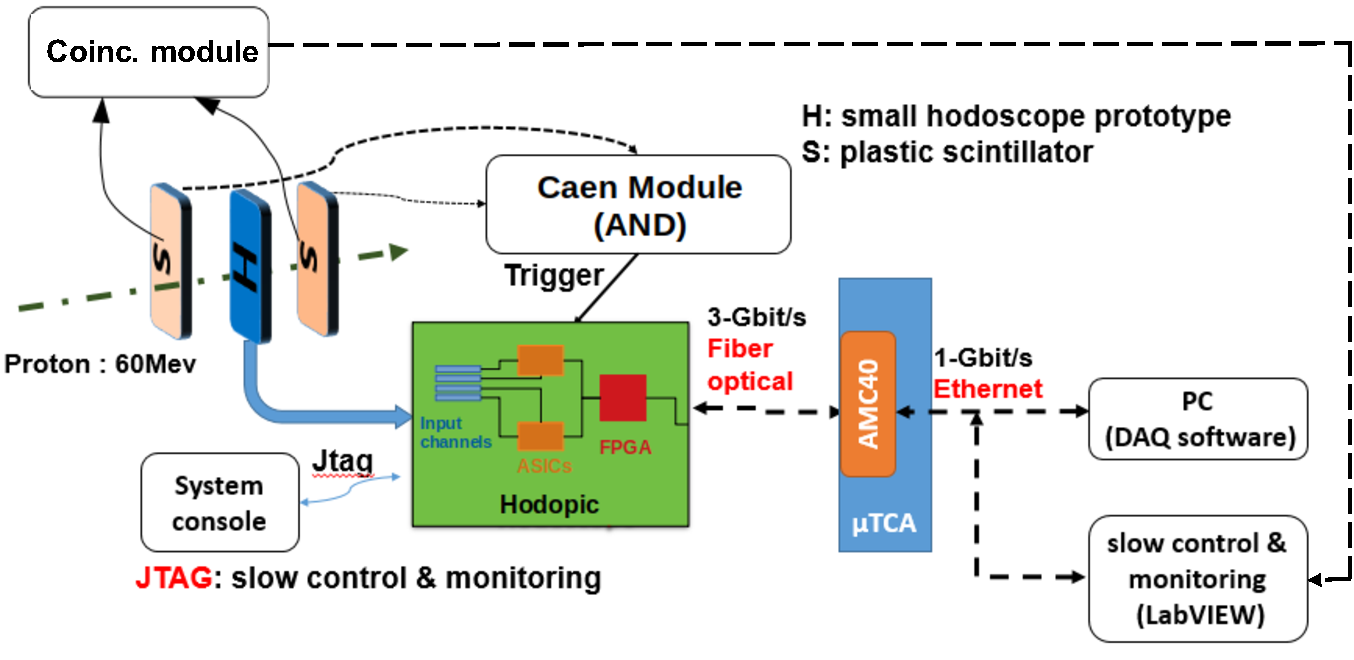
\includegraphics[width=1\textwidth]{figures/Scheme_Setup_Nice_08_2019.pdf}
\caption{\small{\textit{Scheme of the data acquisition chain of the experimental setup.}}}
\label{fig:Scheme_Setup_hodo}
\end{figure} 

In order to monitor the ageing of the fibers, another data acquisition mode has been foreseen in which the signal amplitude of a given channel is measured by means of an ADC implemented in the ASIC.

For this study, a smaller hodoscope with 32 fibers per plane has also been developed in order to use a single acquisition board to collect all the data of the two planes. Each fiber plane is readout by a single ASIC.

Overall, the data acquisition parameters of the hodoscope are the following: the PM high-voltage and the ASIC gains and thresholds. As detailed in section~\ref{sec:Settings}, these parameters can be optimized in order to improve the data collection and improve the signal-to-background ratio.


\subsection{General principle of the experimental setups}
\label{GeneralPrinc}

Figure \ref{fig:Picture_Setup_hodo} illustrates the setup used to assess the performances of the hodoscope during in-beam tests. The external trigger signal is provided by the coincidence signal generated from two plastic scintillators (PS) when a proton impinges the hodoscope. This trigger replaces the one generated by the gamma camera in the final PG detection device of the CLaRyS collaboration.

The fact that these detectors are slighlty larger than the beam hodoscope does not matter since we have verified that the whole beam crosses the hodoscope (Figure~\ref{fig:2D_Maps} in the Results section). PS are aligned with the beam and located about 5~cm upstream and downstream of the hodoscope. Their signals are read out by PM which are connected to a Nuclear Instrumentation Module (NIM) where the analog signals are converted into logic signals via a preset threshold. This configuration allowed us to generate double (two PS) and triple coincidences (two PS AND the beam tagging hodoscope: either the OR or the AND of the two planes). The ratio of the number of triple and double coincidences is a direct measure of the detector efficiency. Since PS counting rate capability is around {10}$^{5}$~Hz, an additional detector is required to monitor larger beam intensities (section~\ref{In-beam_tests}).

\begin{figure}[htb]
\centering
\includegraphics[width=0.5\textwidth]{figures/Experimental_setup_hodoscope_March_August_2019_marked.pdf}
\caption{\small{\textit{Typical experimental setup used to assess the performances of the hodoscope during in-beam tests. The two plastic scintillators are used in order to provide an external trigger signal when a proton impinges the hodoscope.}}}
\label{fig:Picture_Setup_hodo}
\end{figure}


\subsection{GANIL experiments}

The radiation damage assessment was performed with the small hodoscope (32 fibers per plane), connected to a single Hamamatsu multi-anode PM biased at 800~V. The setup described in the previous section was used to measure the hodoscope efficiency.  

The PM readout was performed with various NIM modules to provide trigger signals (discriminator module), charge integration (QDC module) and timing (TAC module)\footnote{QDC: charge-to-digital converter : TAC: time-to-digital concerter.}. The discriminator threshold was set at 30~mV, which corresponds to about one sixth of the maximum of the amplitude distribution. The effect of radiation damage was estimated by measuring detection efficiency after a few irradiation periods with high beam intensity.

\subsection{Centre Antoine Lacassage (CAL) experiments}
\label{In-beam_tests}

In addition to the setup described in section~\ref{GeneralPrinc}, a third PS has been installed out of the beam irradiation field in order to monitor the beam intensity in high beam intensity conditions. This detector was calibrated with the in-beam PS at low beam intensity and with the intensity measured in the cyclotron stripper at high intensities. 

Moreover the three single independent signals and the coincidence module output signal were sent to the LabView-based program to visualize the various counting rates and to provide online monitoring of the beam intensity. 
Finally, the time selection window applied in the FPGA of the FE card before data transmission was tuned from an additional PC through a JTAG link.

The MEDICYC low energy treatment line of the CAL is intended for the treatment of ocular tumors. The research area of this beam line is located a few meters upstream of the treatment room. The maximum beam energy is 64.5~MeV and the high frequency of the accelerator is 24.85~MHz so that the beam consists of proton bunches arriving every 40.24~ns. Throughout the rest of the paper, beam intensities are expressed in Hz because the mean number of protons per bunch is always below 1 for the range of intensities used during these experiments. The counting rates recorded in the PS are approximated to Hz unit.
The performance of the hodoscope is mainly assessed in terms of detection efficiency and spatial resolution. The number of hit fibers per trigger (multiplicity) and the detection profiles are also considered in this characterization study.

\subsection{Criteria and settings}
\label{sec:Settings}

As mentioned in section~\ref{sec:hodo}, the data acquisition parameters of the hodoscope are the PM high-voltage and the ASIC gains and thresholds. Their settings aim at finding the best compromise between noise rejection and detection efficiency.

The standard method consists in measuring the so-called S-curves obtained by means of a logic periodic signal sent to each input channel, one by one. The S-curve corresponds to the numbers of pulses detected by the FE card over a given acquisition time as a function of threshold. Actually two types of events can be distinguished according the various signals provided by the ASIC, namely the logic signals associated to each channel and the request signal (logical OR of all channels):
\begin{itemize}
  \item Good events (GE): events for which at least one logic signal state is high, 
  \item Event with short pulse (ESP): undesired events for which logic signal is not long enough to have a high state when the reading of the channel states by the FPGA is requested by the ASIC (see section~\ref{sec:hodo}).
\end{itemize}

Figure~\ref{fig:S_Curve} presents the S-curves measured for a gain of 1.50. As expected the GE curve presents a plateau (the expected number of pulses over the acquisition time) up to the sharp fall-off for threshold values close to the signal amplitude (point B). In this fall-off region the larger the threshold the smaller the probability to have long enough logic signals to be readout by the FPGA. This is the reason why the ESP curve presents a maximum at the bottom of the GE curve fall-off. Finally the peak observed in the ESP curve for very low threshold values (below point A) is due to the electronics noise. The interval defined by points A and B corresponds to the suitable threshold range (STR) for a given channel gain.

The method used to determine a set of gains and threshold is based on three main steps:
\begin{itemize}
	\item A first scan of the input channels consists in determining the noisiest channel for the minimal gain (0.25), i.e.~the channel for which point A (in figure \ref{fig:S_Curve}) corresponds to the largest threshold value. Points A and B of this channel are then used as a reference STR ;
	\item The STR of the other channels is then measured for the minimal gain (0.25). The cumulative function of the overlap of this STR with the reference STR is then computed. The maximum of this distribution is defined as the optimal threshold value ;
	\item For channels whose STR has no overlap with the reference STR, the gain is increased step by step until an overlap shows up.
\end{itemize}
%The following beam test was dedicated to assess the correction of an artifact in the firmware impacting the time resolution (cf \ref{Time_resolution}).

\begin{figure}[htb]
\centering
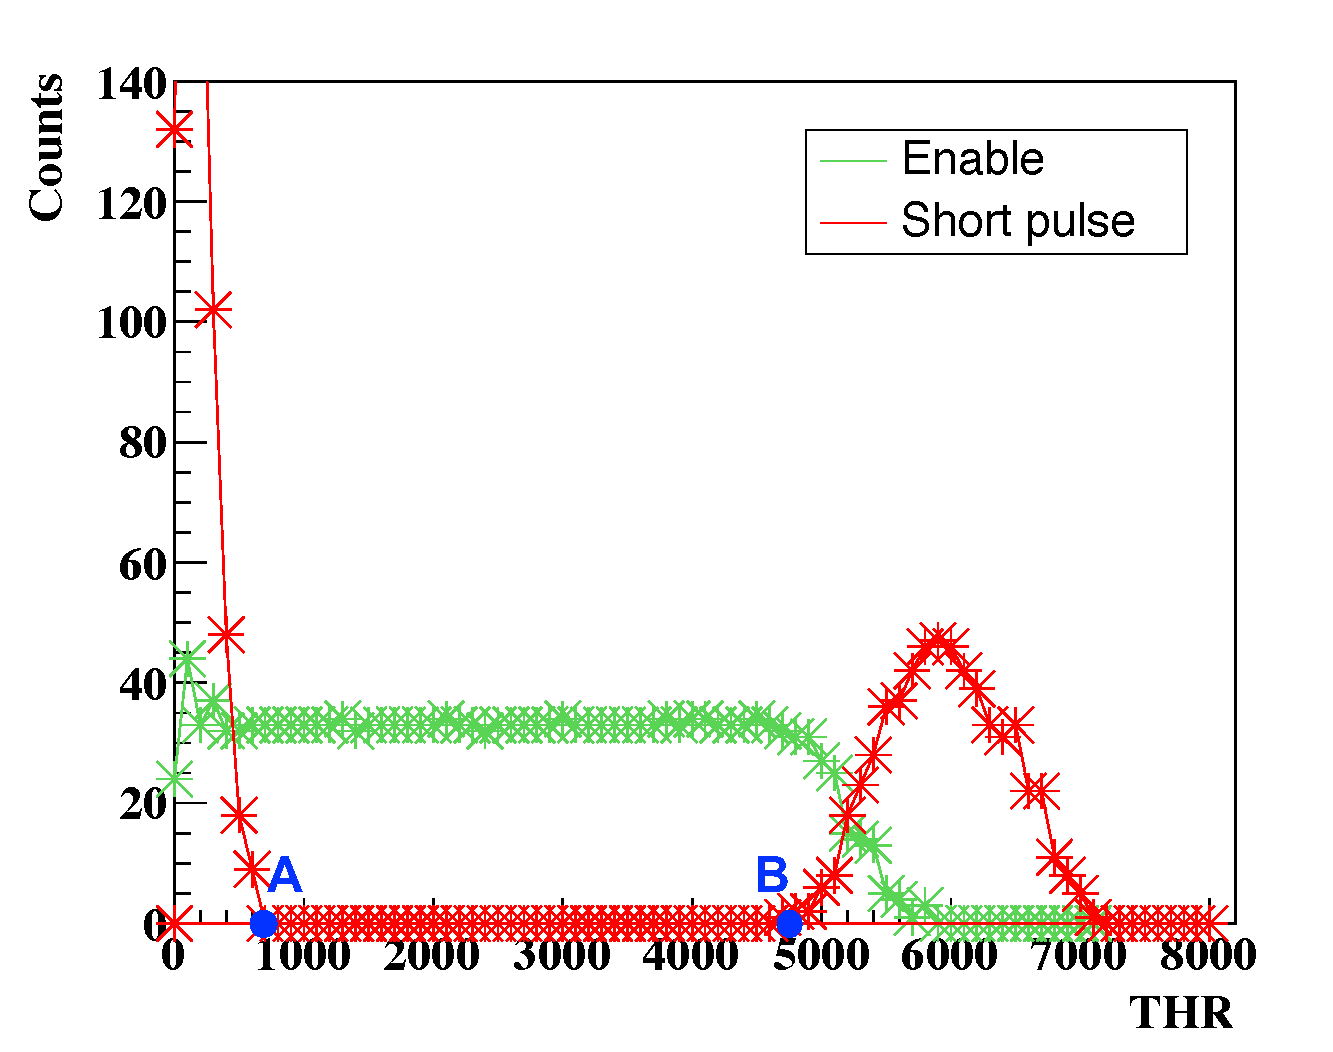
\includegraphics[width=0.5\textwidth]{figures/S_Curve_Thr_suitable_rangeAB.pdf}
\caption{\small{\textit{Number of \enquote{good events} (GE) and \enquote{events with short pulse} (ESP) events as a function of the threshold (THR) for a given channel. The range between points A and B corresponds to a suitable threshold range for this channel.}}}
\label{fig:S_Curve}
\end{figure}

Finally the cross-talk between neighboring pixels has been assessed by scanning the PMs with a blue LED. Although slightly larger than the provider specifications, the cross-talk measured with our setup always remains below 3\% which is sufficiently low to be easily rectified by an adapted threshold setting \cite{FontanaPhD}.

\section{Results}
\subsection{Experiment with carbon ions at GANIL}
A total detection efficiency of 94\% was obtained with a single plane, while the fraction of events with multiplicity > 1 represented 24\%, mainly due to cross talk between adjacent channels of the multi-anode PM.
From SRIM estimation \cite{Ziegler2010}, the energy deposit in a 1~mm thick plastic fiber is 26~MeV. The results for the integrated charge per projectile, and the measured efficiency, are reported in Table~\ref{tab:GANIL}. A significant decrease of the efficiency was measured after 2.2$\times$10$^{12}$~ions$\cdot$cm$^{-2}$, but it was almost recovered by lowering the threshold. 
Close to 90\% detection efficiency was kept after 3.6$\times$10$^{12}$ ions$\cdot$cm$^{-2}$.
Concerning the irradiation damages, it should be noted that after few days, a partial restoration of the response at laboratory test benches has been observed, but it was not possible to repeat the detection efficiency measurement with carbon ions. 
The time resolution was measured between one fiber output and the cyclotron high frequency signal, and assessed to 550~ps RMS. 
\begin{table}[htb]
\caption{\small{\textit{Evolution of the hodoscope response as a function of 95~MeV/u carbon ion fluence. The detection efficiency is measured on a single fiber plane with a multi-anode PM H8500 and a power supply of 800~V. A threshold of 30~mV corresponds to 4.5~pC measured on QDC.}}}
\centering
\begin{tabular}{|c|c|c|c|c|c|}
\hline
Fluence (cm$^{-2}$)& 0 & (7.2$\pm$1.2)$\times$10$^{11}$ & (2.2$\pm$0.4)$\times$10$^{12}$ & (2.2$\pm$0.4)$\times$10$^{12}$ & (3.6$\pm$0.7)$\times$10$^{12}$\\
\hline
\makecell{Discriminator\\threshold (mV)} & 30 & 30 & 30 & 15 & 15\\
\hline
\makecell{Mean QDC\\value (pC)} & 35 & 34 & 27 & 21 & 21\\
\hline
Efficiency (\%) & 94 & 94 & 63 & 92 & 86\\
\hline
\end{tabular}
\label{tab:GANIL}
\end{table}

\subsection{Experiments with protons at CAL}
\subsubsection{Profiles and multiplicities}
\label{Profiles_And_Multiplies}

The event multiplicity ($M$) is defined as the number of involved fibers per plane when a trigger is generated. Figure \ref{fig:Multiplicity} presents the distributions of multiplicity $P(M)$ of both planes for three beam intensities: 17~kHz, $\sim$1.3~MHz and $\sim$20~MHz. The mean number of protons per bunch is 6.8$\times$10$^{-4}$, 5.2$\times$10$^{-2}$ and 8.0$\times$10$^{-1}$ respectively. The Poisson distribution of the number of protons per bunch for bunches consisting of at least 1 proton is superimposed for each beam intensity since it corresponds to the expected multiplicity if we neglect the multiple proton arrivals in a single fiber. $P(M = 0)=0$ since bunches without proton do not trigger the data acquisition. 

At low beams intensities (17~kHz and $\sim$1.3~MHz), we measured $P(M=1)$ values of 80\% and 70\% for X and Y planes respectively, to be compared to the expected value of 100\%. Experimental events with $M=0$ corresponds to empty events including events with short pulse (ESP) (section~\ref{sec:hodo} and \ref{sec:Settings}). Events with $M\ge2$ are probably due slight ground fluctuations in the ASICs leading to multiple hit channels (with \enquote{wrong hits}) while only one fiber has been crossed by an incident proton. 

At 20~MHz, the effect of ground fluctuations is amplified. Indeed, although the detection efficiency ($P(M\ge1)$ remains almost constant, the experimental distribution of multiplicity significantly deviates from the expected distributions. Further improvement of the ASIC are therefore required to be compliant with beam intensities used clinical centers.

\begin{figure}[htb]
\centering
    \begin{subfigure}{0.32\textwidth} \centering 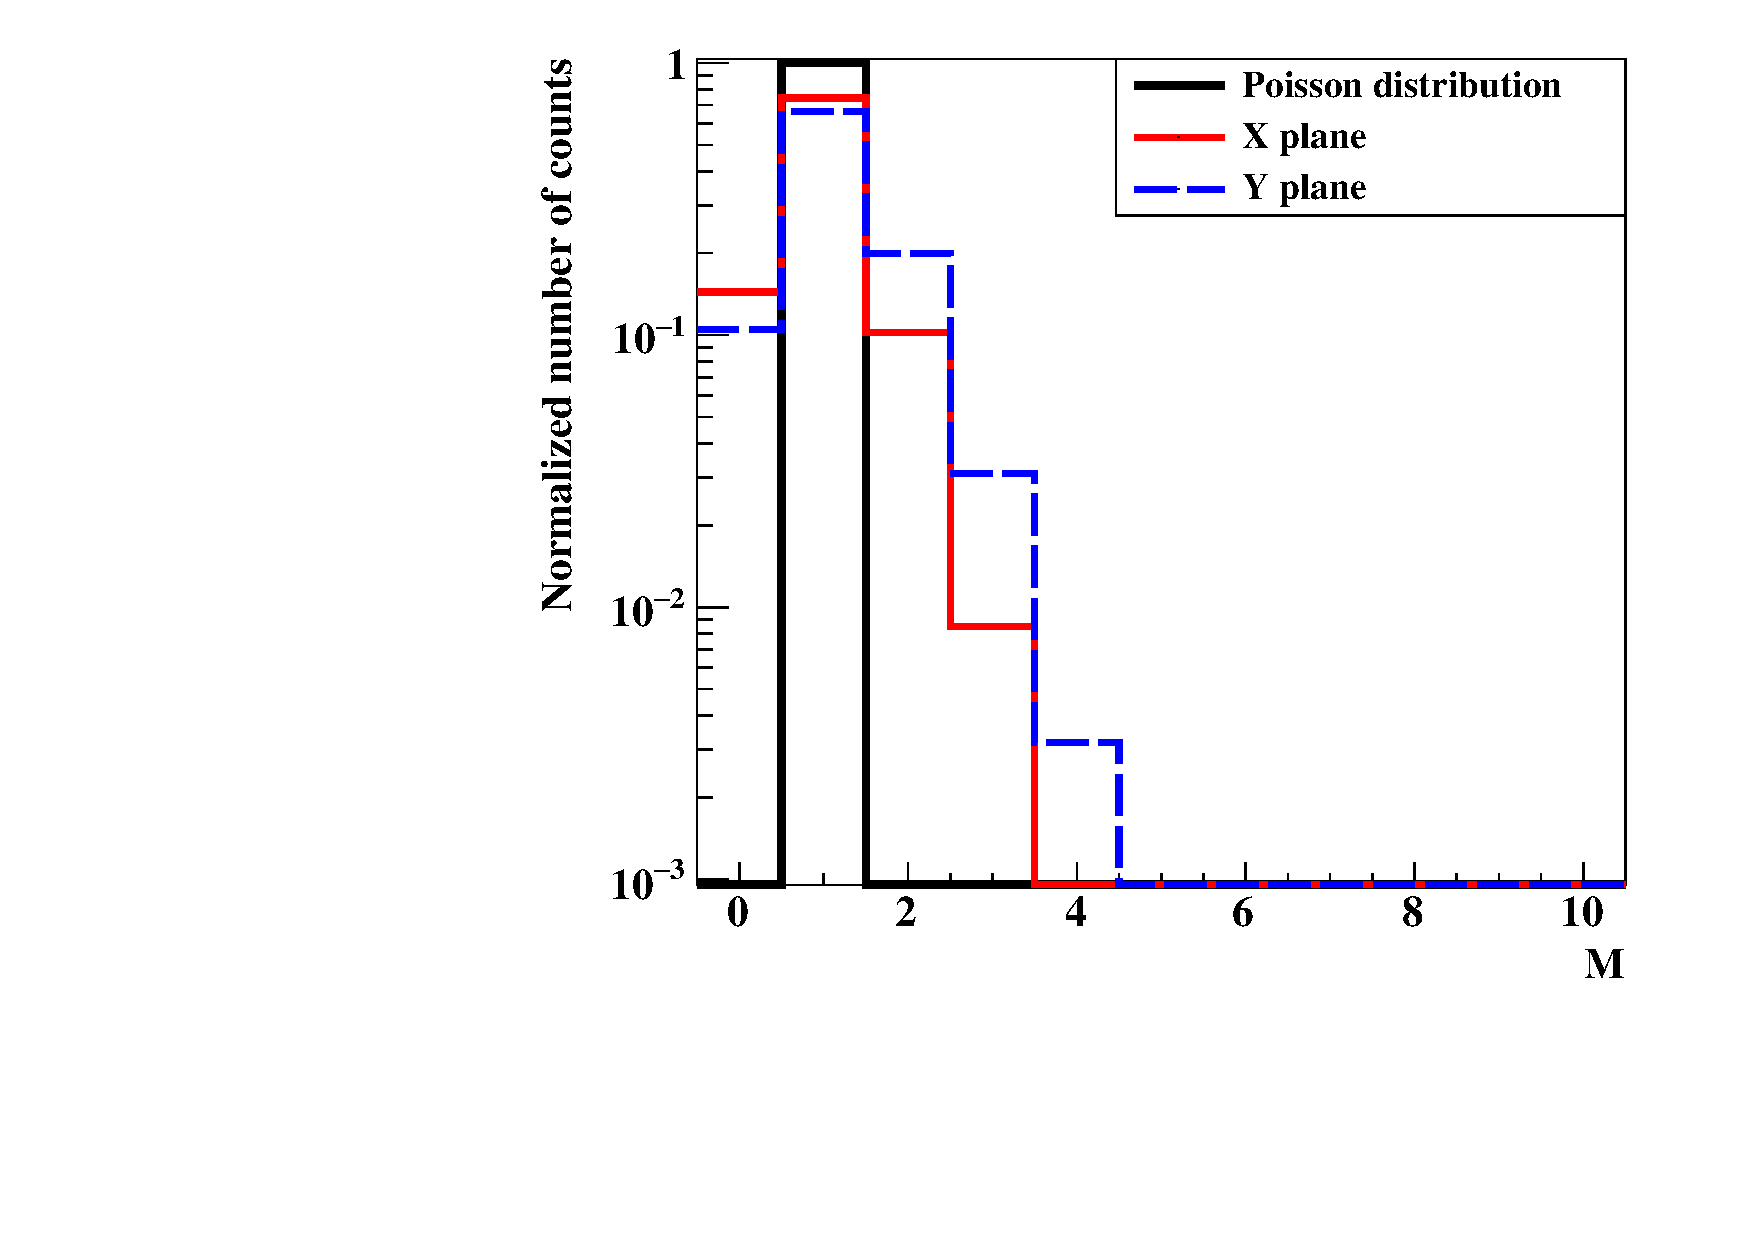
\includegraphics[width=\textwidth]{figures/Involved_fibers_17kHz_without_X=0.pdf} \caption{} \label{fig:Fibers_17kHz}
    \end{subfigure}
    \begin{subfigure}{0.32\textwidth} \centering 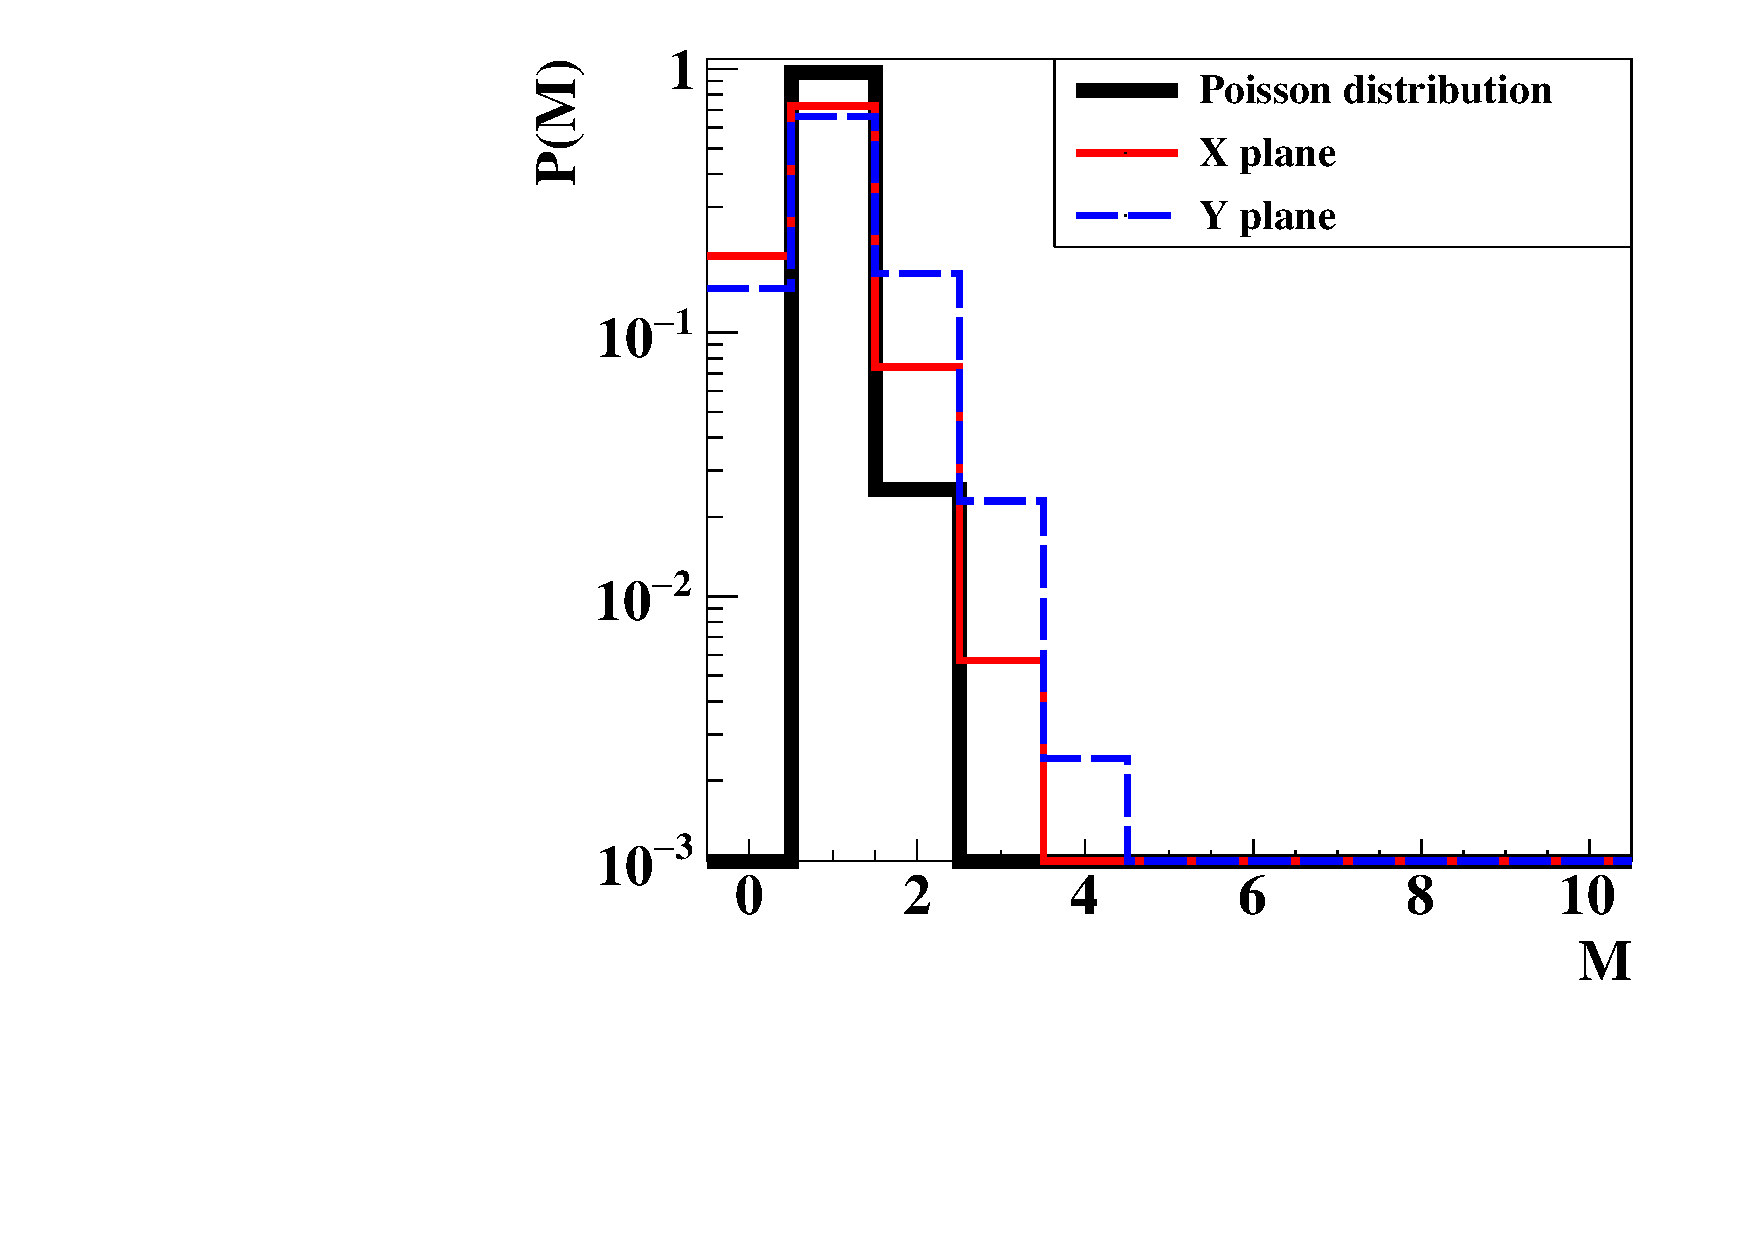
\includegraphics[width=\textwidth]{figures/Involved_fibers_1MHz_without_X=0.pdf} \caption{} \label{fig:Fibers_1MHz}
    \end{subfigure}
    \begin{subfigure}{0.32\textwidth} \centering 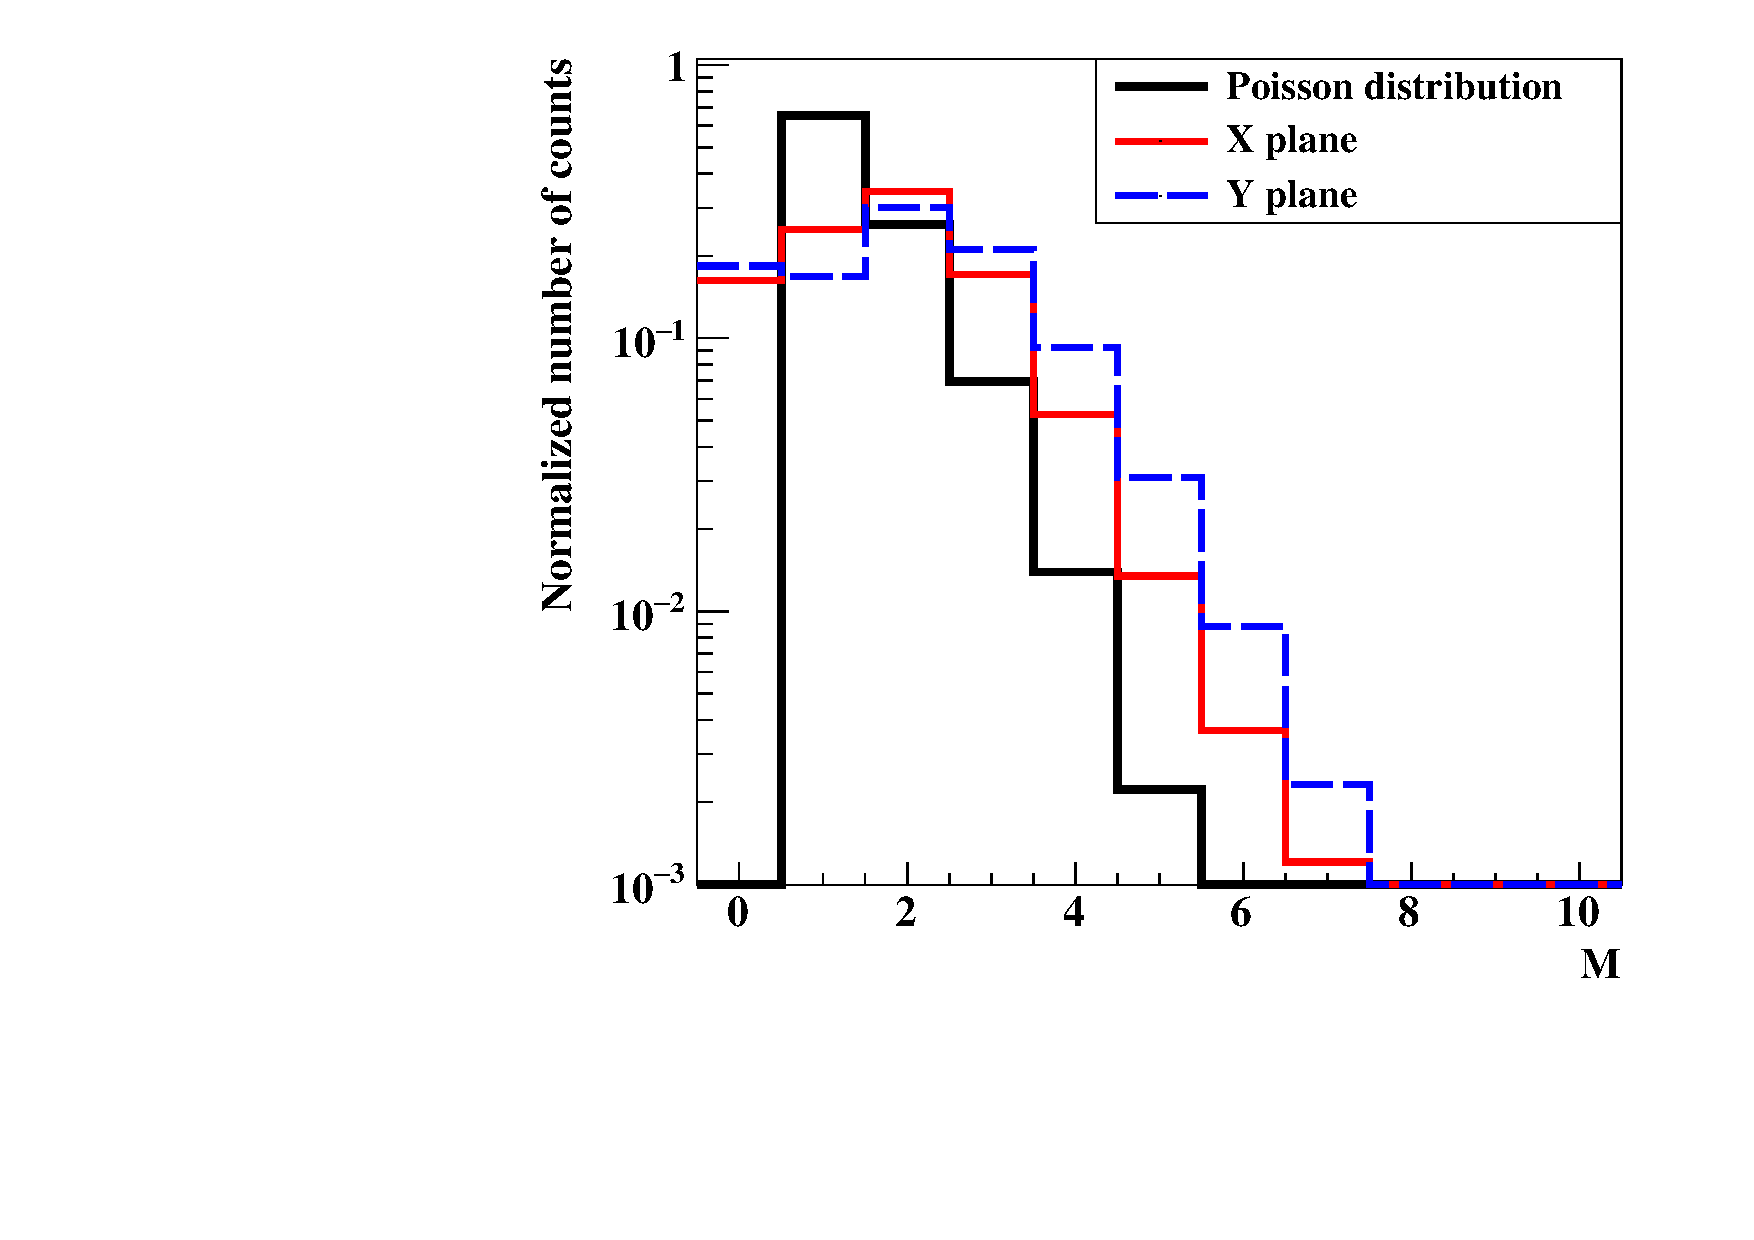
\includegraphics[width=\textwidth]{figures/Involved_fibers_20MHz_without_X=0.pdf} \caption{} \label{fig:Fibers_20MHz}
    \end{subfigure}
\caption{\small{\textit{Distribution of event multiplicity $P(M)$ for beam intensity of (a) 17~kHz, (b) $\sim$1.3 MHz and (c) $\sim$20 MHz.}} }
\label{fig:Multiplicity}
\end{figure}

The monitoring software reconstructs two-dimensional maps for each acquisition. Figure~\ref{fig:2D_Maps} represents maps obtained for two acquisitions at 17~kHz and $\sim$20~MHz. The reconstruction method uses the  average position in X and Y for events with $M > 1$. Although the shape of the beam varies between the two intensities, the center of the beam is clearly defined. The shape modification is attributed to the change of the focusing lens of the beam when the intensity increases. 

\begin{figure}[htb]
\centering
    \begin{subfigure}{0.45\textwidth} \centering 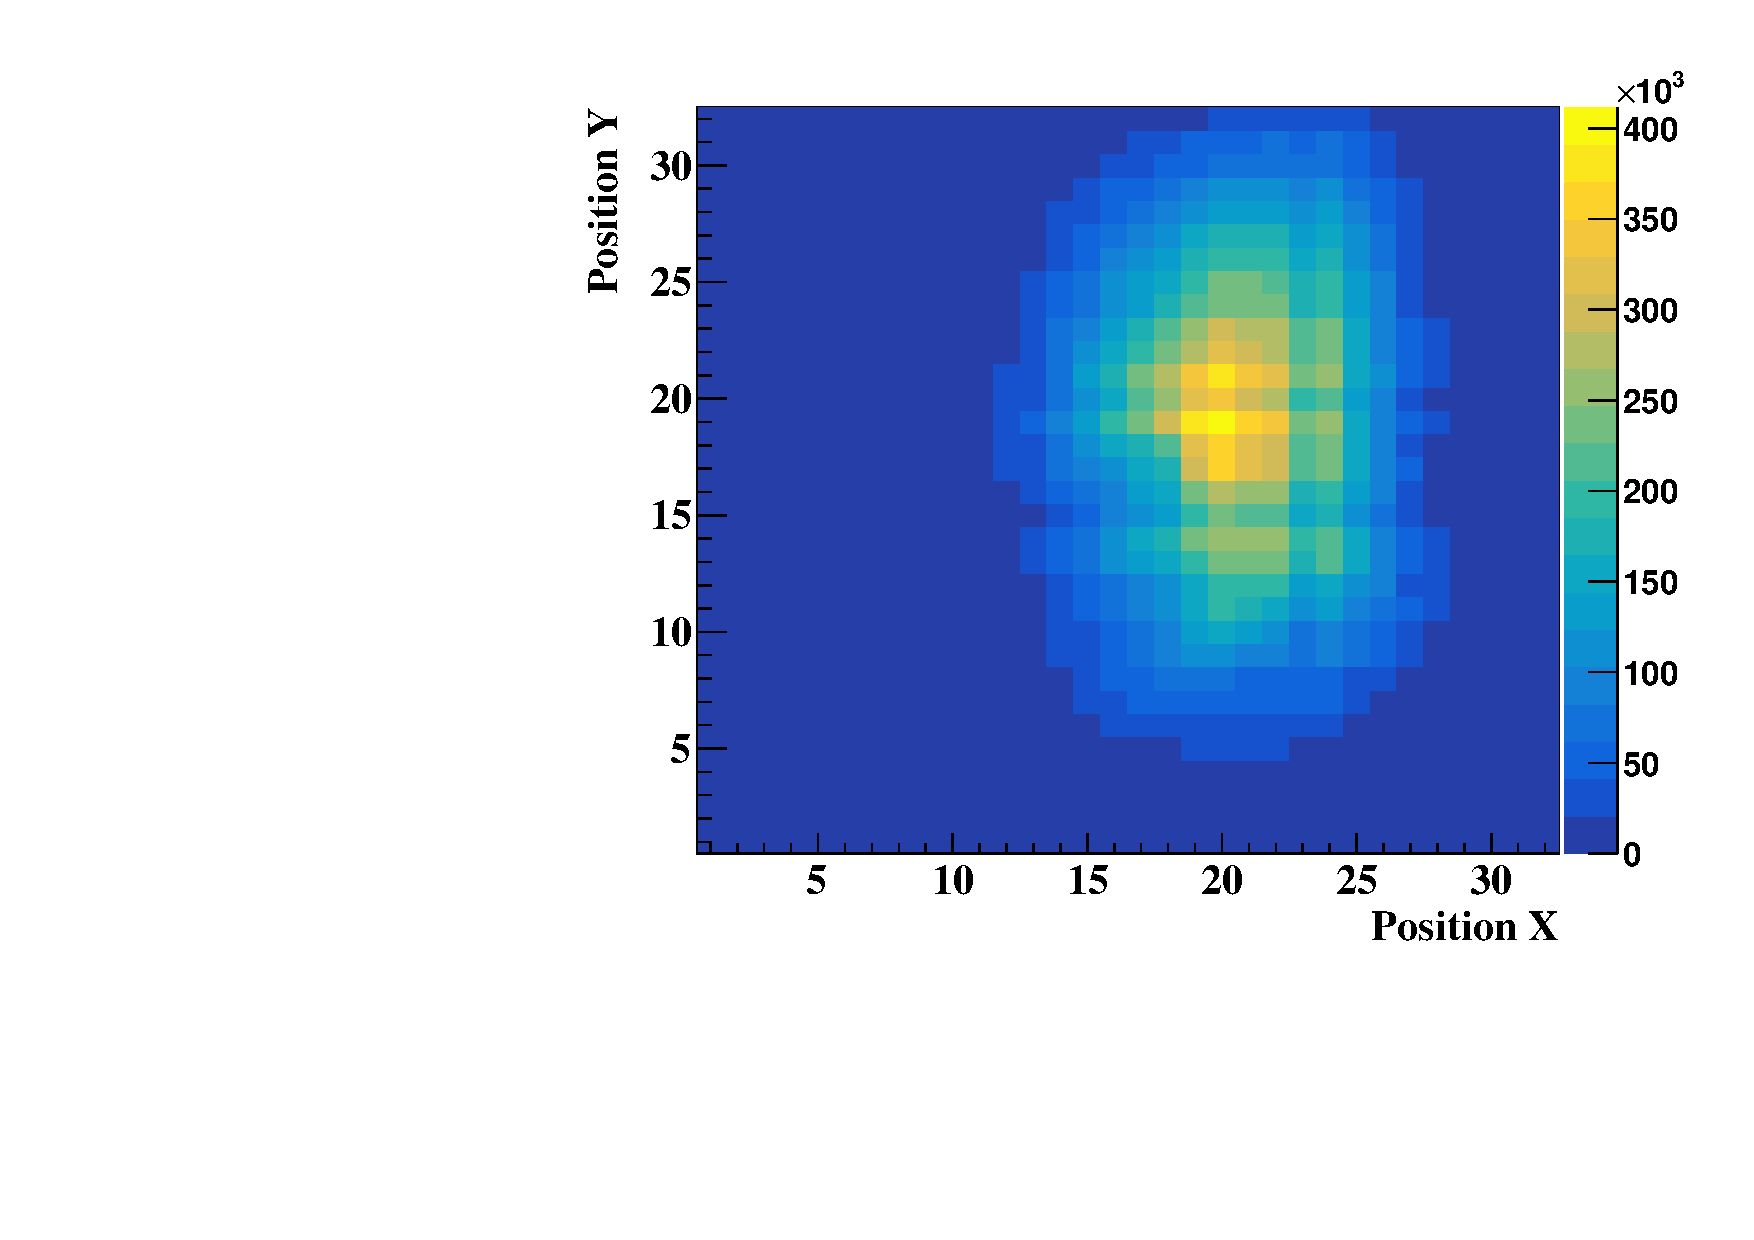
\includegraphics[width=\textwidth]{figures/2D_Map_1MHz.pdf} \caption{} \label{fig:2D_1MHz}
    \end{subfigure}
    ~
%\newline
%\centering
    \begin{subfigure}{0.45\textwidth} \centering 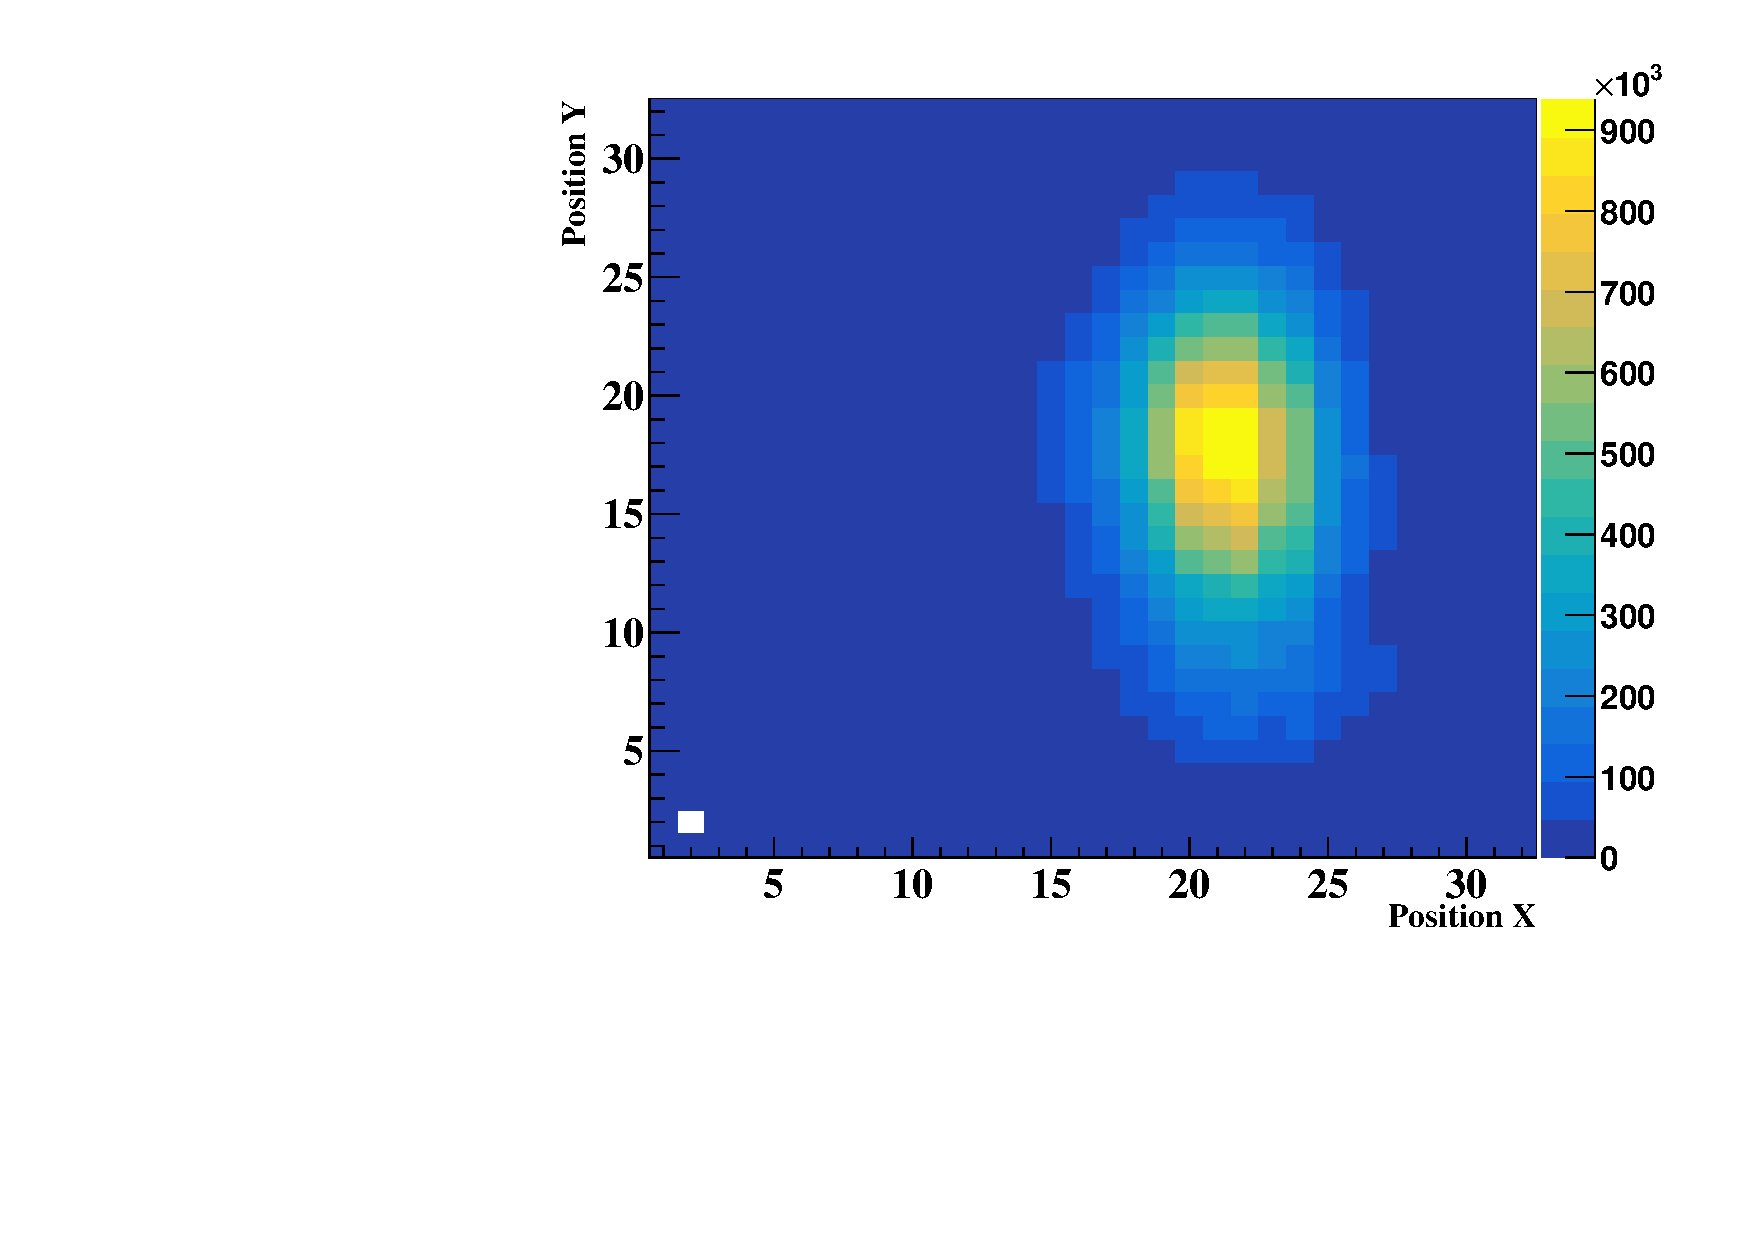
\includegraphics[width=\textwidth]{figures/2D_Map_20MHz.pdf} \caption{} \label{fig:2D_20MHz}
    \end{subfigure}
\caption{\small{\textit{2D map reconstruted from data collection for a beam intensity of (a) $\sim$1.3 MHz and (b) $\sim$20 MHz.}}}
\label{fig:2D_Maps}
\end{figure}

Figure \ref{fig:1D_Profiles} represents the X and Y profiles obtained with two events selection methods for the irradiation with a beam intensity of $\sim$1.3~MHz. The blue curves correspond to the method used  for the 2D map reconstruction (average position of events with M>1) while the red curve has been obtained with the selection of $M=1$ events. The good overlap between the curves in both planes confirms that the method used for the 2D map reconstruction is adapted. However, for intensities larger than $\sim$20~MHz, the overlap of the two curves is lost due to the increase of \enquote{wrong hits} (not shown).

\begin{figure}[htb]
\centering
    \begin{subfigure}{0.47\textwidth} \centering 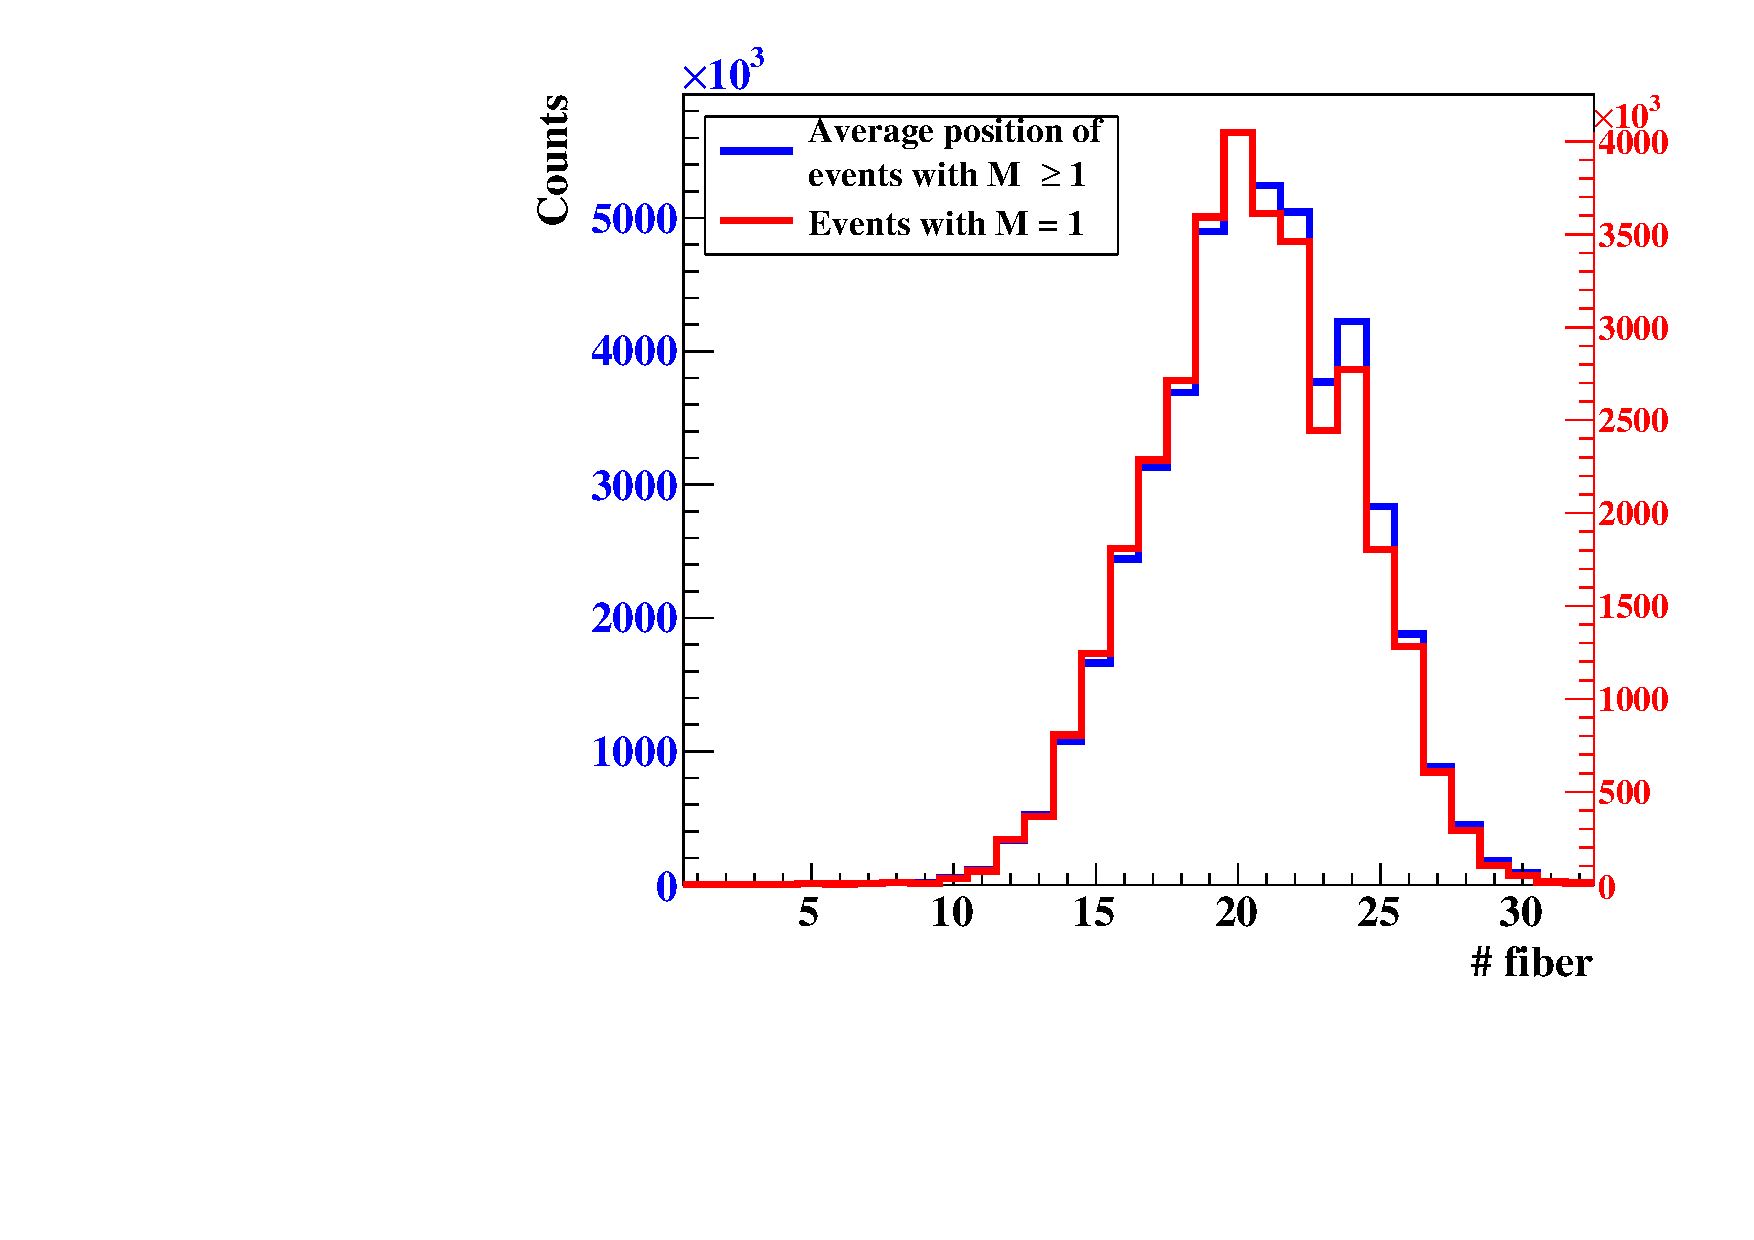
\includegraphics[width=\textwidth]{figures/Plane_X_1MHz.pdf} \caption{} \label{fig:Plane_X_1MHz}
    \end{subfigure}
    ~
    \begin{subfigure}{0.47\textwidth} \centering 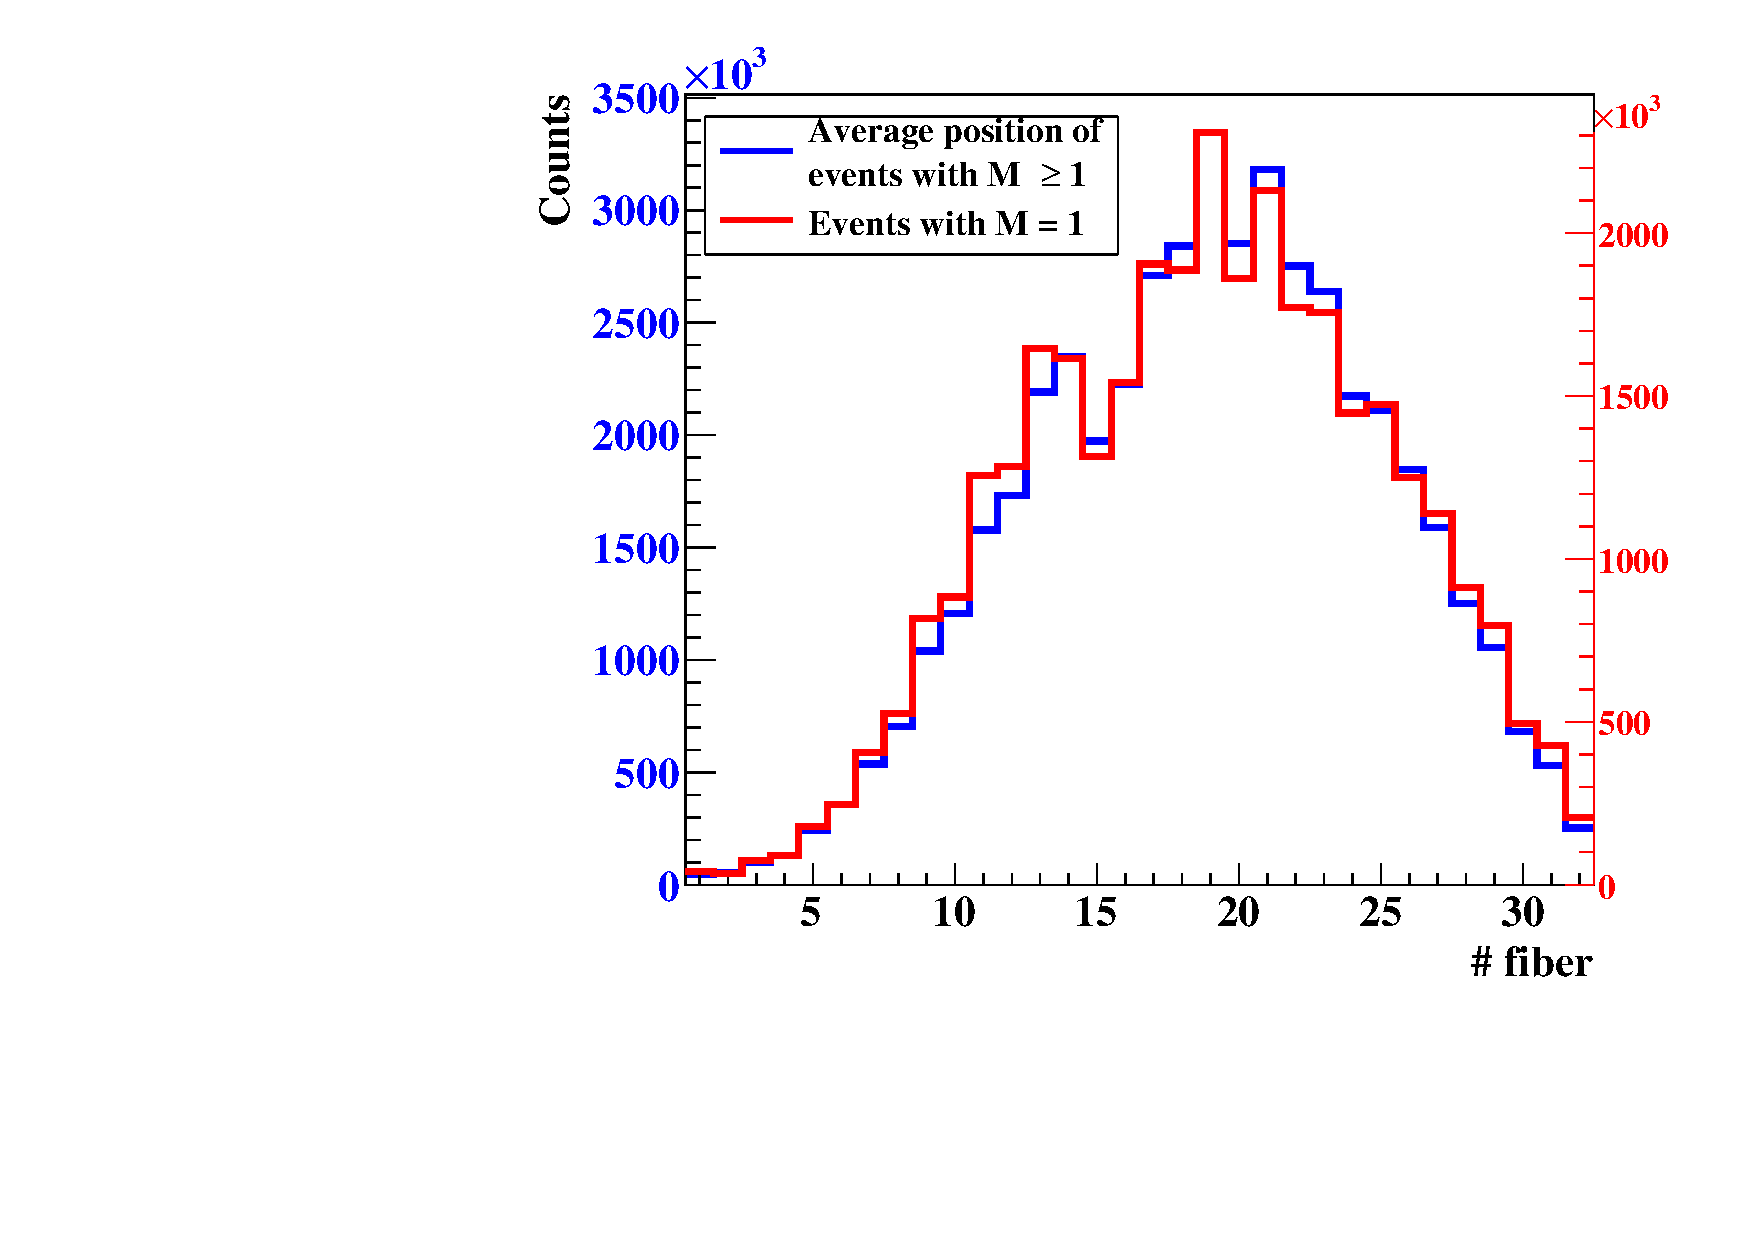
\includegraphics[width=\textwidth]{figures/Plane_Y_1MHz.pdf} \caption{} \label{fig:Plane_Y_1MHz}
    \end{subfigure}
\caption{\small{\textit{1D profiles of (a) X and (b) Y fiber planes with multiplicity M=1 and M$\geq$1 for a beam intensity of $\sim${1.3}~MHz.}}}
\label{fig:1D_Profiles}
\end{figure}

Considering that no structure is expected in the beam shape, the structures observed in the 1D profiles are attributed to slightly different efficiencies over the X and Y planes. The order of magnitude of these differences has been assessed focusing on the fibers obviously under-responding, namely fiber 23 in X plane and fibers $(15,16)$ and 20 in Y plane. Applying a linear interpolation over these fibers, we derived an estimate of the efficiency loss due to these fibers. In overall the loss increases with the beam intensity from 0.75\% to 4\% (resp.~2.7\% to 4\%) in the X (resp.~Y) plane.  

\subsubsection{Detection efficiency}

Figure \ref{fig:DE} represents the detection efficiency of X and Y planes separately and with logical OR and AND conditions on the data of both planes for various intensities from 2~kHz to $\sim$20~MHz. The data are corrected for under-responding channels (cf. \ref{Profiles_And_Multiplies}). The detection efficiencies in X and Y planes keep almost constant values around 84\% and 90\% respectively for intensities under $\sim$6~MHz. They result in a coincidence detection efficiency (logical AND between X and Y fibers) close to 74\% while the logical OR condition on both planes provides a detection efficiency close to 100\% in the same range of intensities. A significant fall-off of detection efficiency is observed at $\sim$20~MHz due to current ASIC limitations, especially ground fluctuations leading to data acquisition retriggering and therefore dead time.   

\begin{figure}[htb]
\centering
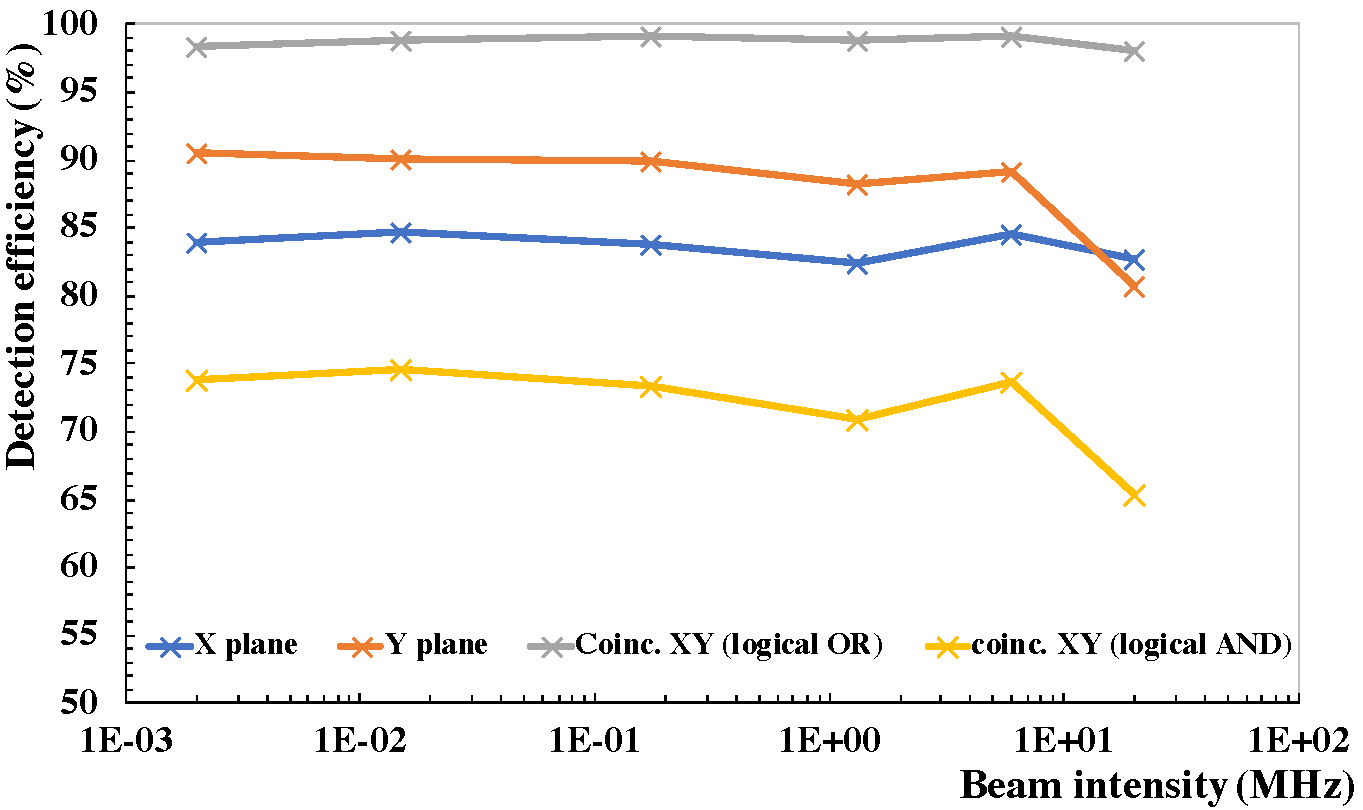
\includegraphics[width=0.7\textwidth]{figures/DE_March_2019_corr.pdf}
\caption{\small{\textit{Hodoscope  detection  efficiency  as  a  function  of the proton beam intensity. A correction factor has been applied to take into account the loss of efficiency due to under-responding channels (see section~\ref{Profiles_And_Multiplies}).}}}
\label{fig:DE}
\end{figure}

\subsubsection{Time resolution}

Figure~\ref{fig:Time_coinc} shows the distributions of time difference between the trigger signal and the first logic signal associated to each fiber planes (X and Y planes)  for beam intensities of 43~kHz (\ref{fig:Time_43kHza} and \ref{fig:Time_43kHzb}) and $\sim$10~MHz (\ref{fig:Time_10MHz}). The distributions obtained with a beam intensity of 43~kHz present well-defined peaks whose widths have been assessed by means of a Gaussian fit. The measured full widths at half maximum (FWHM) are close to 1.5~ns which fulfills the specifications. The distributions at $\sim$10~MHz reveals an additional component before the main peak that is due to ASIC oscillations. Note that the time distributions are governed not only by the time resolution of the hodoscope but also by the one of the PS detectors which has not been measured.
\label{Time_resolution}

\begin{figure}[htb]
\centering
    \begin{subfigure}{0.3\textwidth} \centering 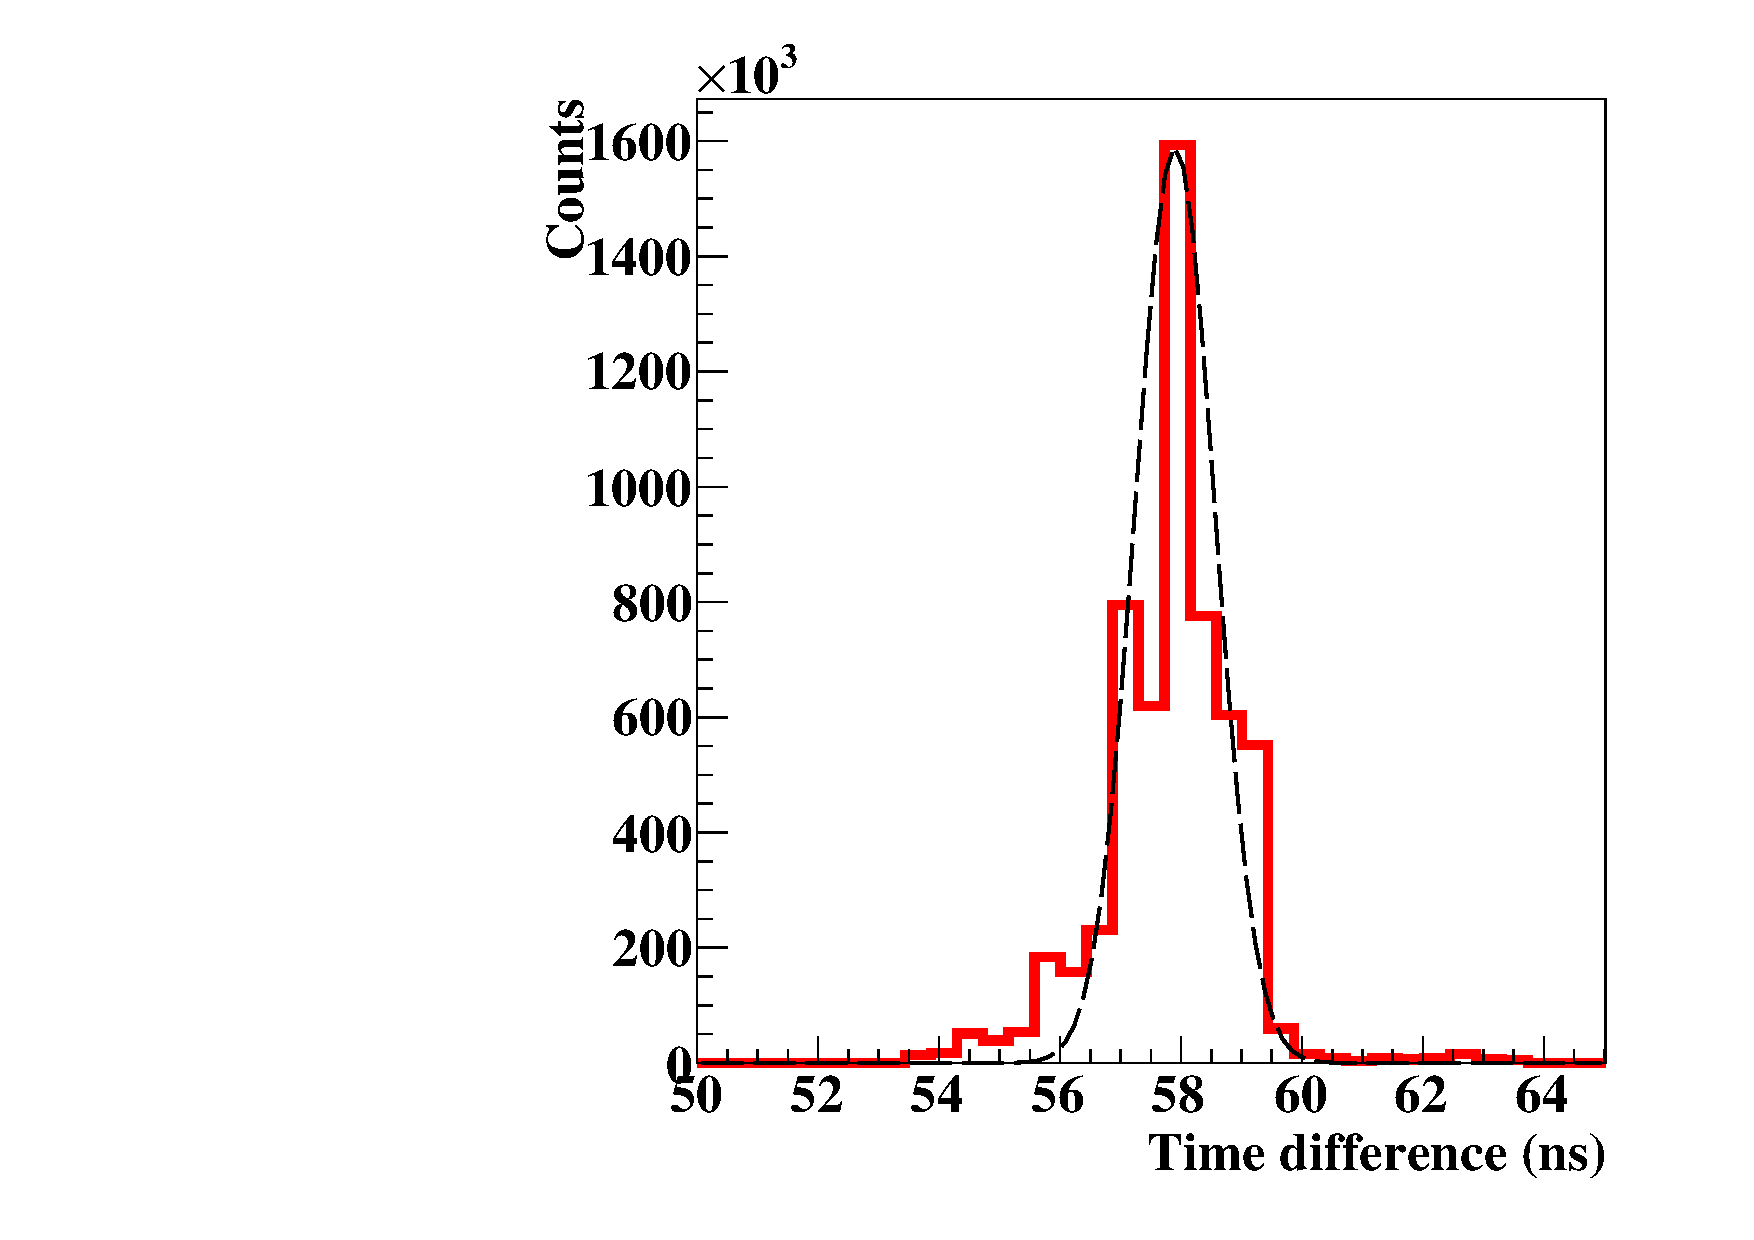
\includegraphics[width=\textwidth]{figures/time_X_43kHz_August.pdf} \caption{} \label{fig:Time_43kHza}
    \end{subfigure}
    ~
    \begin{subfigure}{0.3\textwidth} \centering 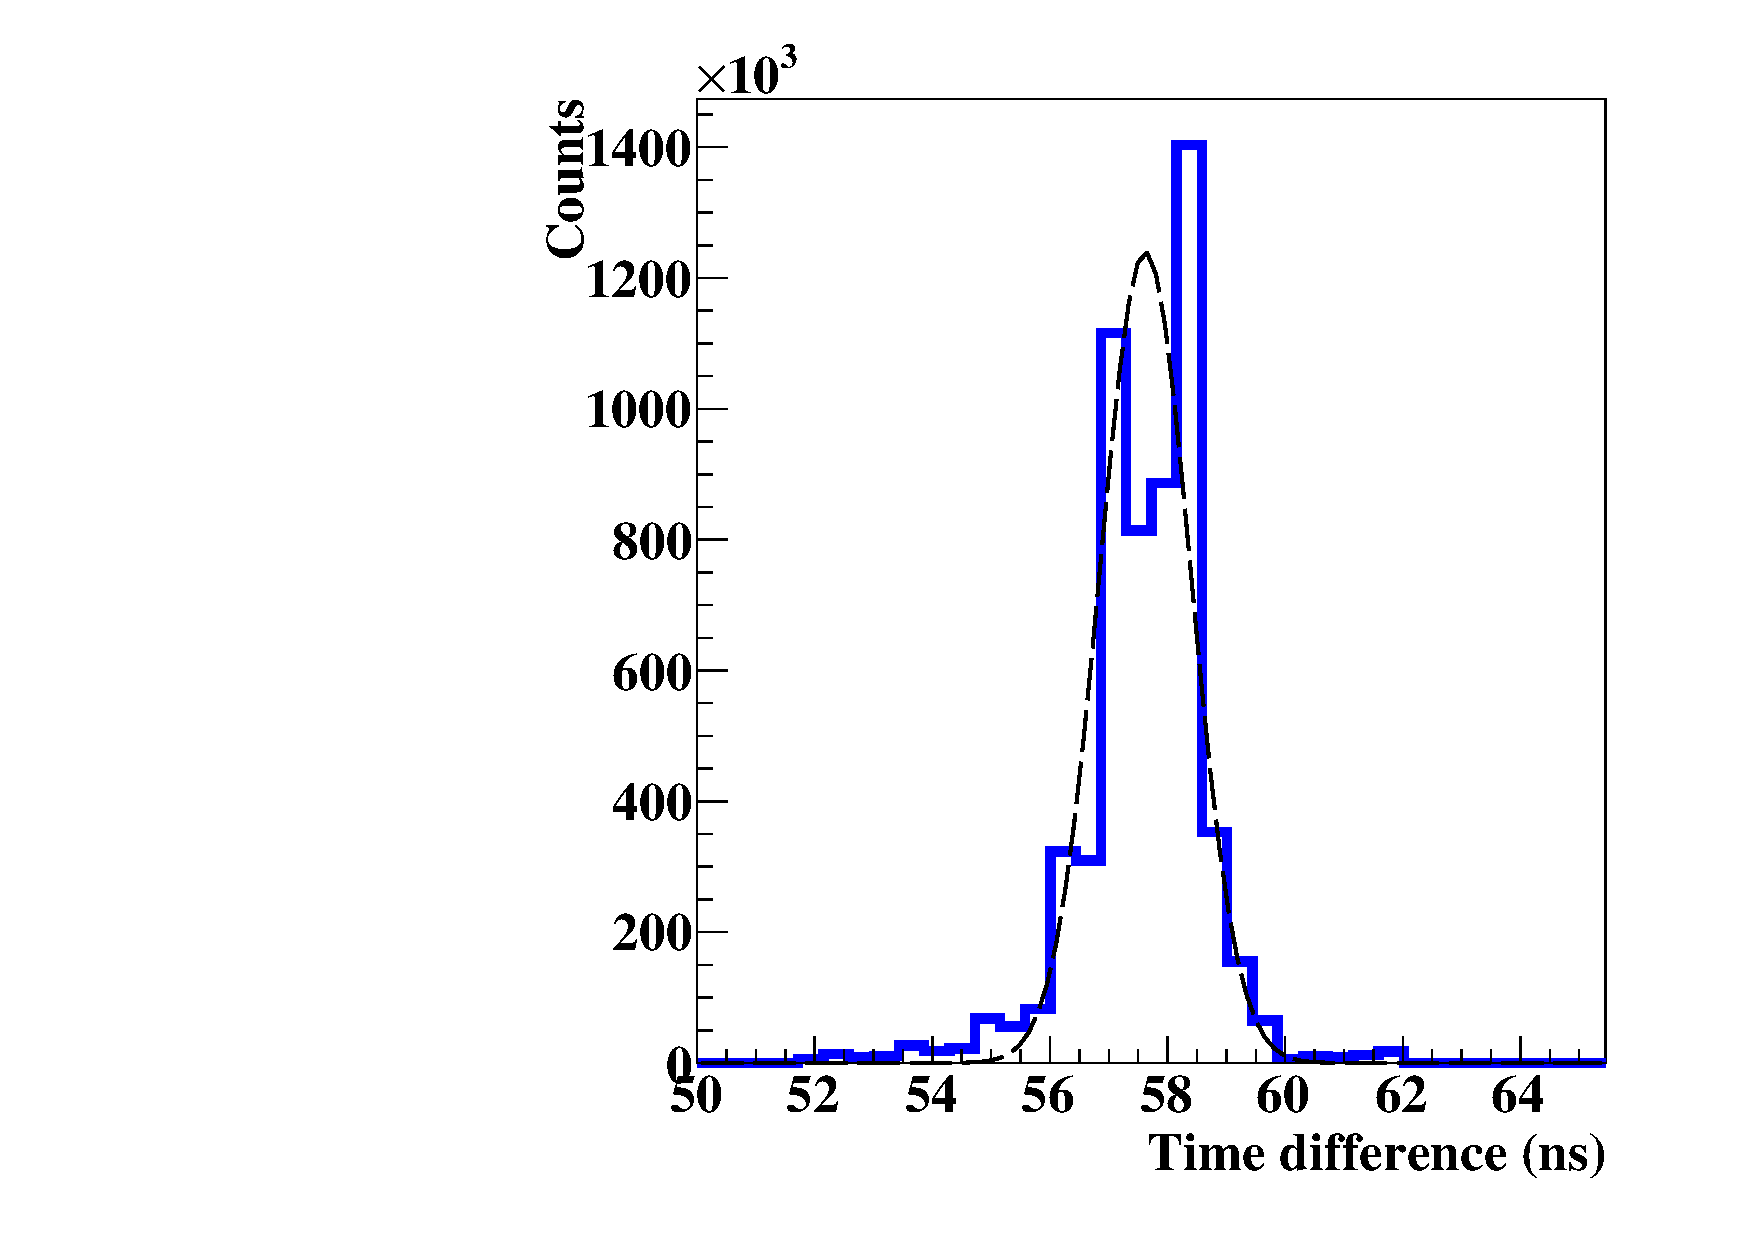
\includegraphics[width=\textwidth]{figures/time_Y_43kHz_August.pdf} \caption{} \label{fig:Time_43kHzb}
    \end{subfigure}    
    ~
%\newline
%\centering
    \begin{subfigure}{0.3\textwidth} \centering 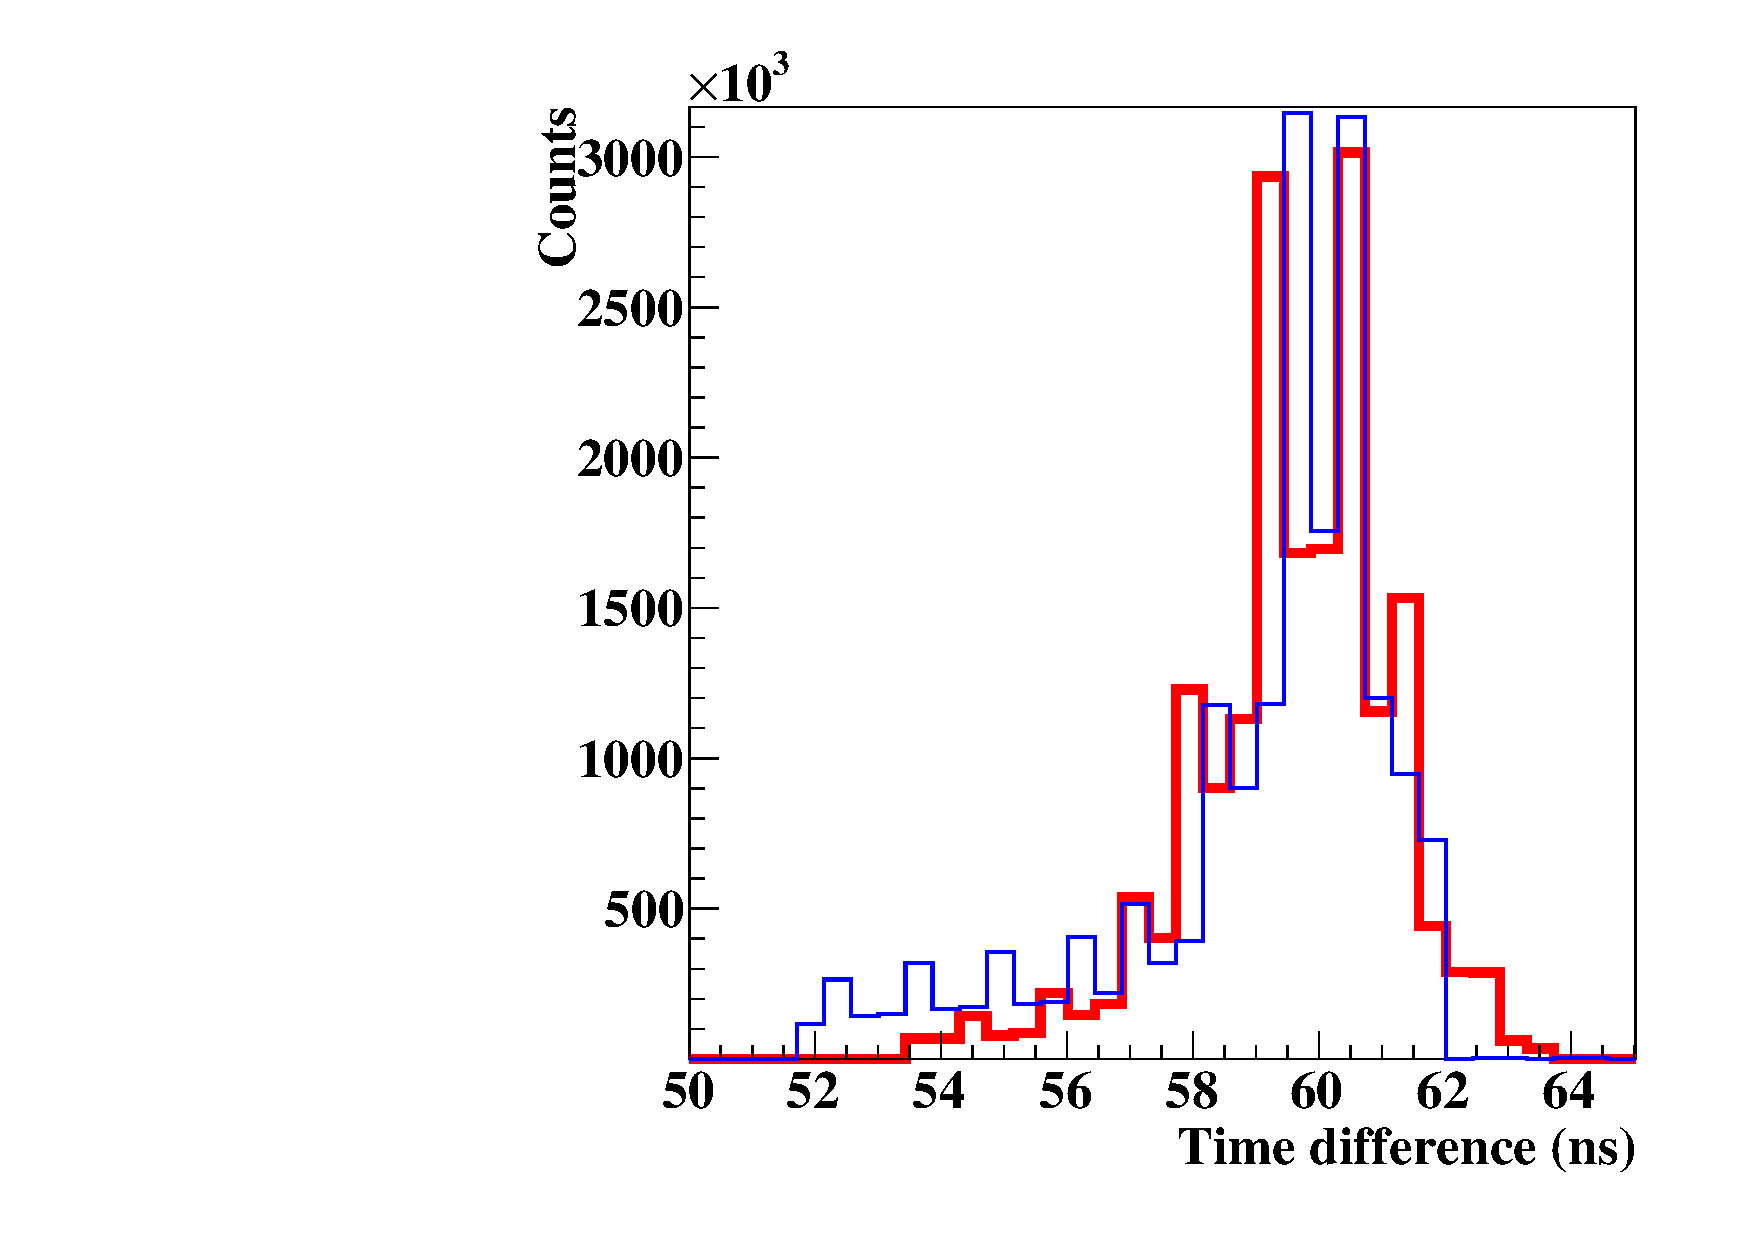
\includegraphics[width=\textwidth]{figures/time_XY_10MHz_August.pdf} \caption{} \label{fig:Time_10MHz}
    \end{subfigure}
\caption{\small{\textit{Distribution of time difference between X and Y fibers (red and blue curves, respectively) and the trigger signal for beam intensities of 43~kHz ((a)--(b)) and $\sim$10~MHz (c).}}}
\label{fig:Time_coinc}
\end{figure}

\section{Discussion}

The beam tagging hodoscope under devolpment intends to provide incident ion detection with an efficiency larger than 90\% with a time resolution below 2~ns FWHM. The life duration of the scintillating fibers should be typically larger that 1000 clinical irradiations and the device should be capable to cope with 100~MHz counting rates expected with beam microstructures encountered in treatment centers. 

Regarding radiation hardness, the experiment performed at GANIL represents the worst case for radiation damage in hadrontherapy (carbon ions with less than 3~cm range in water). During a single irradiation experiment, less than 10\% efficiency decrease was observed with (3.6$\pm$0.7)$\times$10$^{12}$~ions$\cdot$cm$^{-2}$, which represents more than 1000 clinical irradiations for the central hodoscope area, without accounting for the longer time scale recovery. Note that efficiency measurements performed at CAL-Nice used the same hodoscope, with a beam size largely overlapping the GANIL spot impact, years later.

In the mean time significant progresses have been made in the development of front-end electronics and data acquisition system in order to fulfill the specifications in terms of detection efficiency, time resolution and counting rate capabilities. Moreover specific configuration methods of the acquisition boards have been defined. Although the detection efficiency with coincidence between X and Y planes is $\sim 75$\%, it should be noticed that more than 90\% of the incident ions are detected by at least one of the fiber planes. Moreover the timing resolution is slighlty better than the objective of 2~ns FHWM. 

However the current limitations of the \enquote{HODOPIC} ASIC prevent us from reaching the counting rate of 100~MHz defined in the specifications. These limitations are probably due to ground oscillations in the ASICs that especially lead to fake channel hits. Such hits have been showed in the experimental distributions of multiplicities compared to the Poisson distributions of the expected number of incident protons per bunch. They have also been observed in the distributions of time difference measured with a beam intensity of $\sim$10~MHz (figure \ref{fig:Time_10MHz}).


Although the time resolution of the CLaRyS hodoscope is slighlty larger than the one of other prototypes developed worldwide, it is close to the expectations and further improvements can be foreseen with an ASIC upgrade. Moreover the detection efficiency of a single fiber plane is comparable to the one of other prototypes for which the detection efficiency with a logical AND between two planes has not been reported yet. Finally, the ability of the beam tagging hodoscope to be coupled to a beam monitoring device to provide trigger signals with 1~$\upmu$s delay as been recently demonstrated~\cite{Chen2019}.


\section{Conclusion}

The performances of the CLaRyS beam tagging hodoscope have been assessed in terms of radiation damage, event multiplicity, detection efficiency and time resolution during several in-beam tests. A methodology of configuration of the ASIC thresholds and channel gains has been tested and it allowed us to obtain a detection efficiency larger than 98\% with a logical OR and 65\% with a logical AND between X and Y fiber planes as well as a time resolution lower than 2~ns FWHM for intensities under 1~MHz. In overall these performances are in accordance with the state of the art. Further improvements of the \enquote{HODOPIC} ASIC are required to reach the counting rate capability defined in the specifications (100~MHz).

%\appendix
%\section{Example of appendix title}
%Please always give a title also for appendices.





\acknowledgments
This work was partially performed in the framework of Labex PRIMES (ANR-11-LABX-0063) and within the frame of the EU Horizon 2020 project RIA-ENSAR2/MediNet (654 002).  

%\paragraph{Note added.} This is also a good position for notes added after the paper has been written.



\bibliography{hodoscope_biblio}
\bibliographystyle{ieeetr}

% We suggest to always provide author, title and journal data:
% in short all the informations that clearly identify a document.

%\begin{thebibliography}{99}

%\bibitem{a}
%Author, \emph{Title}, \emph{J. Abbrev.} {\bf vol} (year) pg.

%\bibitem{b}
%Author, \emph{Title},
%arxiv:1234.5678.

%\bibitem{c}
%Author, \emph{Title},
%Publisher (year).


% Please avoid comments such as "For a review'', "For some examples",
% "and references therein" or move them in the text. In general,
% please leave only references in the bibliography and move all
% accessory text in footnotes.

% Also, please have only one work for each \bibitem.


%\end{thebibliography}
\end{document}
